\documentclass[UTF8]{ctexbeamer}
\usepackage{ctex}
\usepackage{beamerthemesplit}
\mode<presentation> {

\usetheme{Madrid}
}

\usepackage{graphicx} % Allows including images
\usepackage{booktabs} % Allows the use of \toprule, \midrule and \bottomrule in tables
\usepackage{fontspec}

% define monaco font
\newfontfamily\Monaco{Monaco}


\title[BLE Security]{BLE环境下的攻击与防范} 

\author{肖心茹 \and 徐文超 \and 杨婧雯} 
\institute[DLUT]
{
大连理工大学软件学院 \\ 
%\medskip
%\textit{https://github.com/knowncold/BLE_Security} % Your email address
\url{https://github.com/knowncold/BLE_Security}
}
\date{\today} 

\begin{document}

\begin{frame}
\titlepage
\end{frame}

\begin{frame}
\frametitle{概览} % Table of contents slide, comment this block out to remove it
\tableofcontents
\end{frame}


\section{概述}

\begin{frame}
  \frametitle{主要工作}
  \begin{itemize}
    \item 了解蓝牙低功耗的工作机制
    \item 了解蓝牙攻击的研究现状
    \item 搭建攻击和实验环境
      \begin{itemize}
      \item iBeacon
      \item YUNMAI Light
      \item MI band 2
      \end{itemize}
    \item 寻找可能的改进方案
  \end{itemize}
\end{frame}

\section{背景}
\subsection{蓝牙}
\begin{frame}
	\frametitle{蓝牙}
	\begin{itemize}
	\item 蓝牙是一种短距离、低功耗的无线网络标准,在计算机和通信设备以及手机、键盘、音频耳机等外围设备中得到了广泛的应用
	\item 蓝牙4.0包含两个标准
		\begin{itemize}
				\item 传统蓝牙,兼容蓝牙1.0,2.0,3.0
				\item BLE是蓝牙低能耗的简称(Bluetooh Low Energy),蓝牙低能耗技术是低成本、短距离、可互操作的鲁棒性无线技术,它利用许多智能手段最大限度地降低功耗
		\end{itemize}
	\end{itemize}
\end{frame}

\begin{frame}
	\frametitle{应用场景}
			\begin{block}{传统蓝牙}
				用于数据量比较大的传输场景,如语音,音乐,较高数据量传输等
			\end{block}
			\begin{block}{低功耗蓝牙}
				应用于实时性要求比较高,但是数据速率比较低的产品,如遥控类的,如鼠标,键盘,遥控鼠标,传感设备的数据发送,如心跳带,血压计,温度传感器等
			\end{block}
\end{frame}

\subsection{蓝牙低功耗}
\begin{frame}
  \frametitle{BLE}
	\begin{figure}
		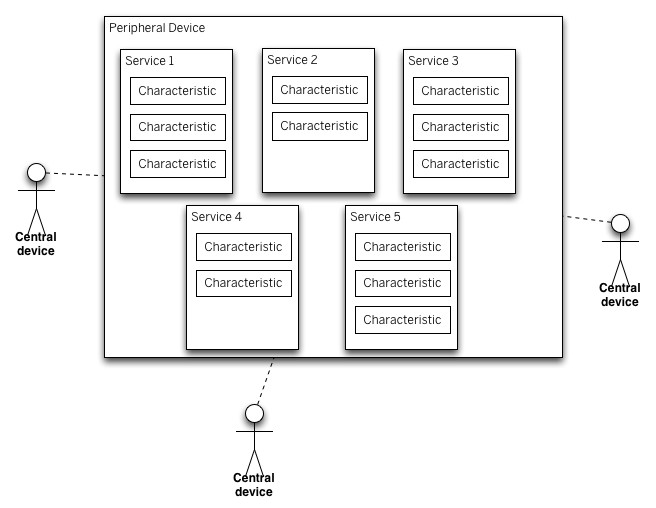
\includegraphics[width=0.7\linewidth]{ble-model.jpg}
	\end{figure}
\end{frame}

\begin{frame}
  \frametitle{BLE}
  \begin{block}{GAP}
Generic Access Profile \\ 控制设备连接和广播,GAP 使设备被其他设备可见,并决定了设备是否可以或者怎样与其他设备交互。例如iBeacon 设备就只是向外广播,不支持连接,小米手环就等设备就可以与中心设备连接。
  \end{block}
  \begin{block}{GATT}
    Generic Attribute Profile \\ 定义两个BLE设备通过Service和Characteristic进行通信。\\
    GATT 连接是独占的,一个BLE外设同时只能被一个中心设备连接;一旦外设被连接,它就会马上停止广播,对其他设备不可见;当中心设备断开,它又开始广播。
  \end{block}
\end{frame}

\subsection{研究现状}
\begin{frame}
	\frametitle{Bluetooth Attack}
	\begin{figure}
		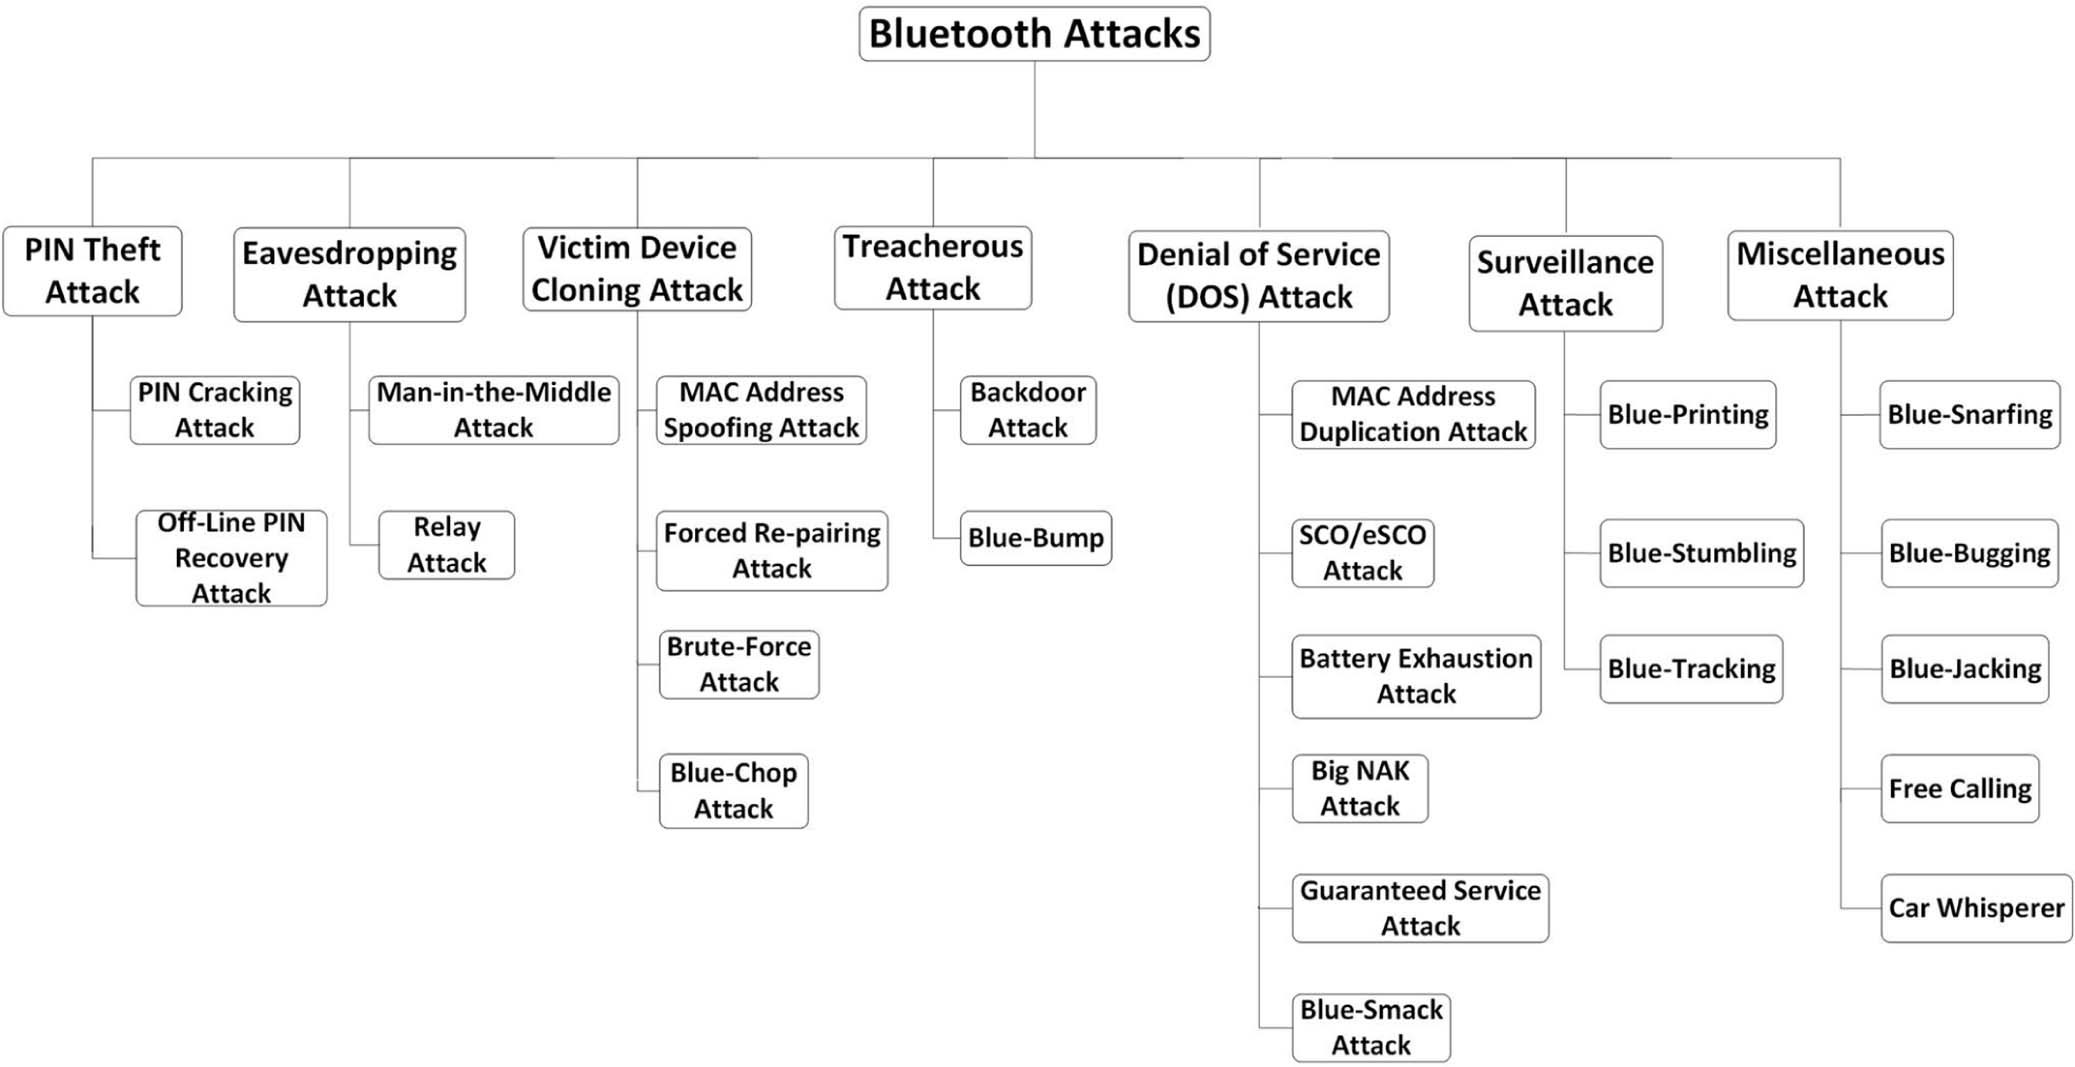
\includegraphics[width=1\linewidth]{bt_attack.jpg}
	\end{figure}
\end{frame}

\section{攻击场景}
\begin{frame}
  \frametitle{使用的工具}
  \begin{alertblock}{软件}
    Kali Linux、hcitool、nRF Connect、nRF Toolbox、LightBlue
  \end{alertblock}
  \begin{alertblock}{硬件}
    云麦好轻体脂秤、小米手环2\\
    Raspberry Pi、TI CC2540、iOS、Android、Arduino 101
  \end{alertblock}
\end{frame}

\subsection{iBeacon}

\begin{frame}
  \frametitle{iBeacon}
  \begin{block}{概述}
    iBeacon是苹果公司2013年9月发布的移动设备用OS(iOS7)上配备的新功能。 \\
    其工作方式是,配备有低功耗蓝牙(BLE)通信功能的设备使用BLE技术向周围以广播形式发送自己特有的ID,接收到该ID的应用软件会根据该ID采取一些行动。
  \end{block}
  \begin{block}{应用场景}
    iBeacon使用BLE技术,成本相当低,作为一项定位技术,有各种各样的应用
    \begin{itemize}
    \item 商场,酒店等推送促销信息。可以定时定点地向客户推送他此时此刻最需要的消息
    \item 机场,体育场,博物馆等推送欢迎消息以及其他客户需要的消息(如航班信息等)
    \end{itemize}
  \end{block}
\end{frame}

\begin{frame}
  \frametitle{iBeacon}
  \framesubtitle{Packet}
  \begin{figure}
    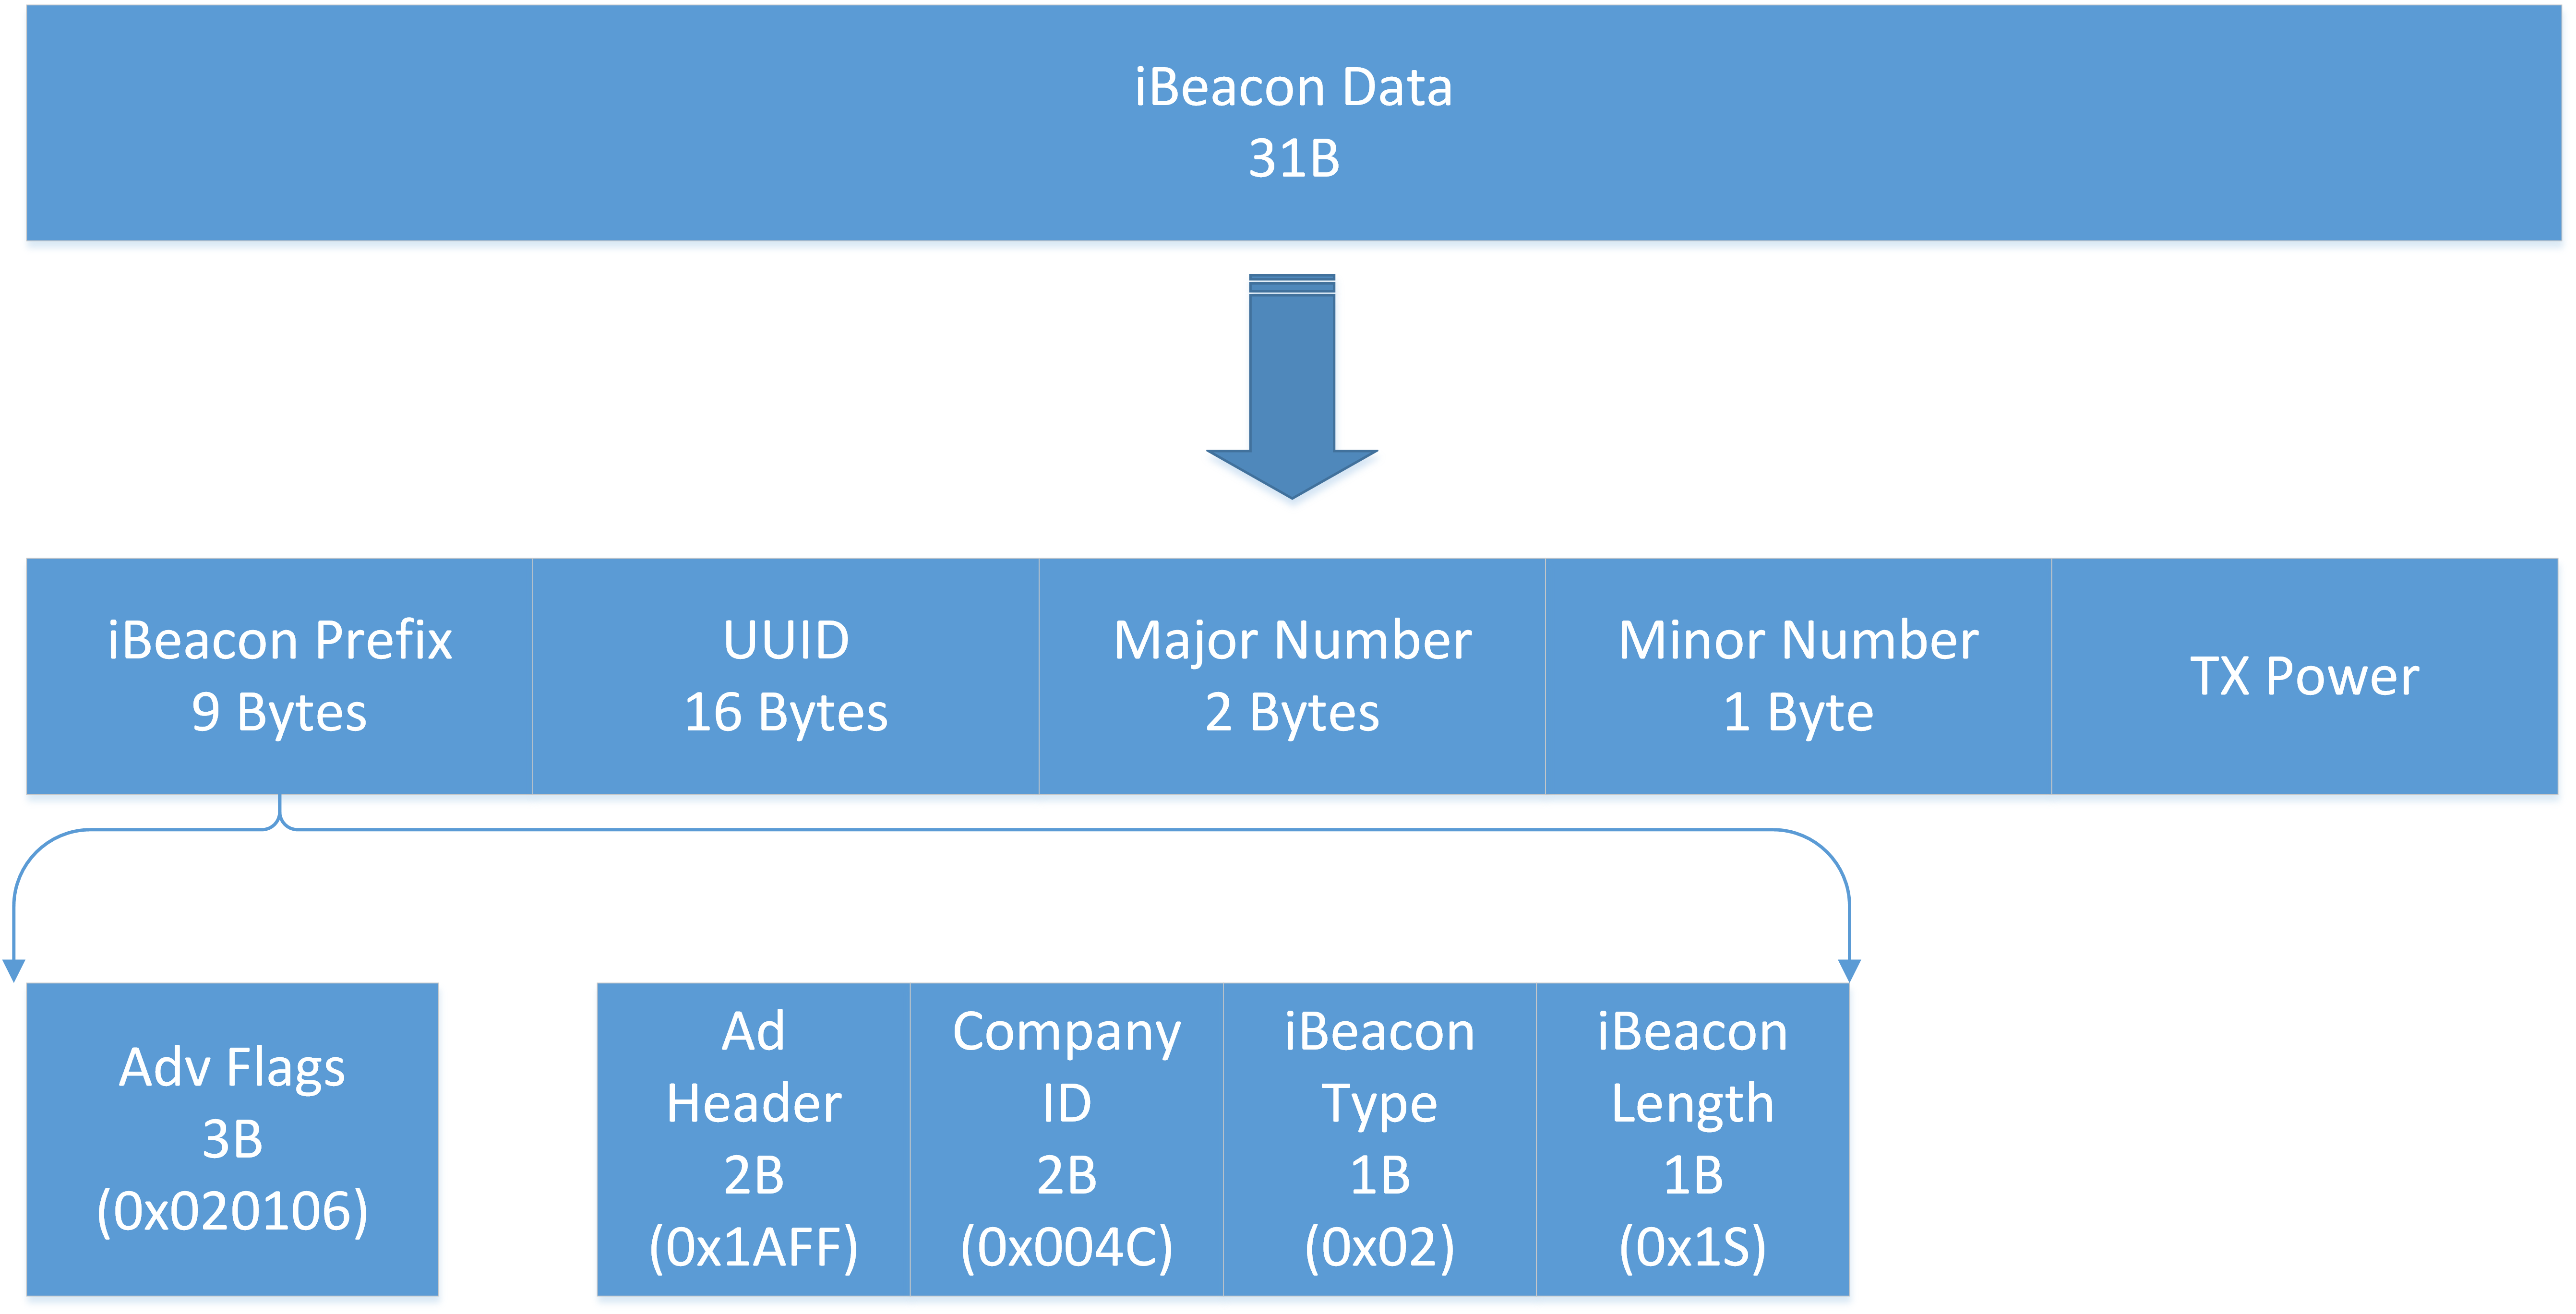
\includegraphics[width=0.9\linewidth]{ibeacon-packet.jpg}
  \end{figure}
\end{frame}

\begin{frame}
  \frametitle{iBeacon}
  \framesubtitle{Attack}
  \begin{block}{嗅探}
    由于使用的是广播的方式,使得嗅探攻击变得十分容易
  \end{block}
  \begin{block}{Spoofing attacks}
    干扰应用的定位,传输错误的信息给云端
  \end{block}
  \begin{block}{}
  由于认证和加密体制的不完善,容易遭受DoS攻击,存在RCE漏洞,存在垃圾邮件的问题
  \end{block}
\end{frame}



\subsection{YUNMAI Light}

\begin{frame}
  \frametitle{YUNMAI Light}
  \begin{columns}
    \column{.5\textwidth}
  \begin{figure}
    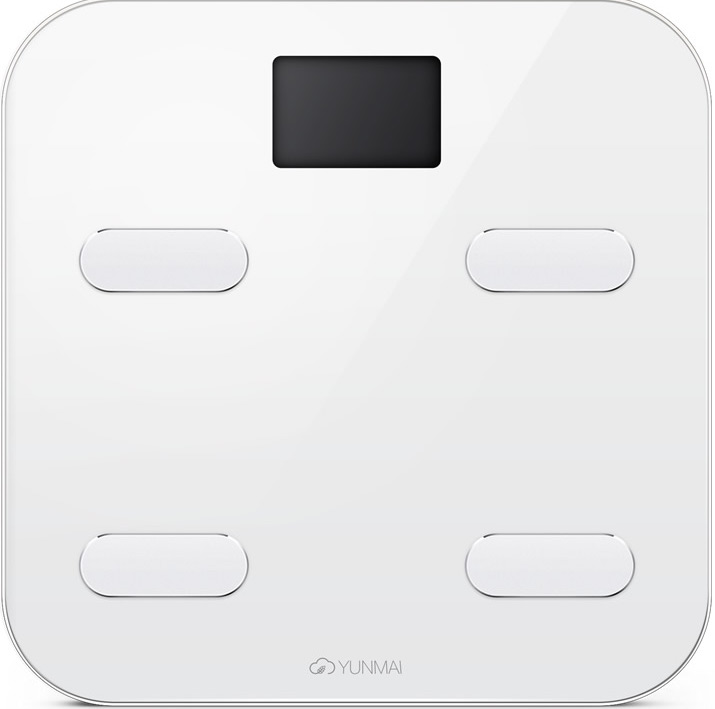
\includegraphics[width=0.9\linewidth]{yunmai-haoqing.jpeg}
  \end{figure}
    \column{.5\textwidth}
  \begin{figure}
    \centering
    \setlength{\fboxrule}{0.001cm}    % 边框线线宽 
    \setlength{\fboxsep}{0}
    \fbox {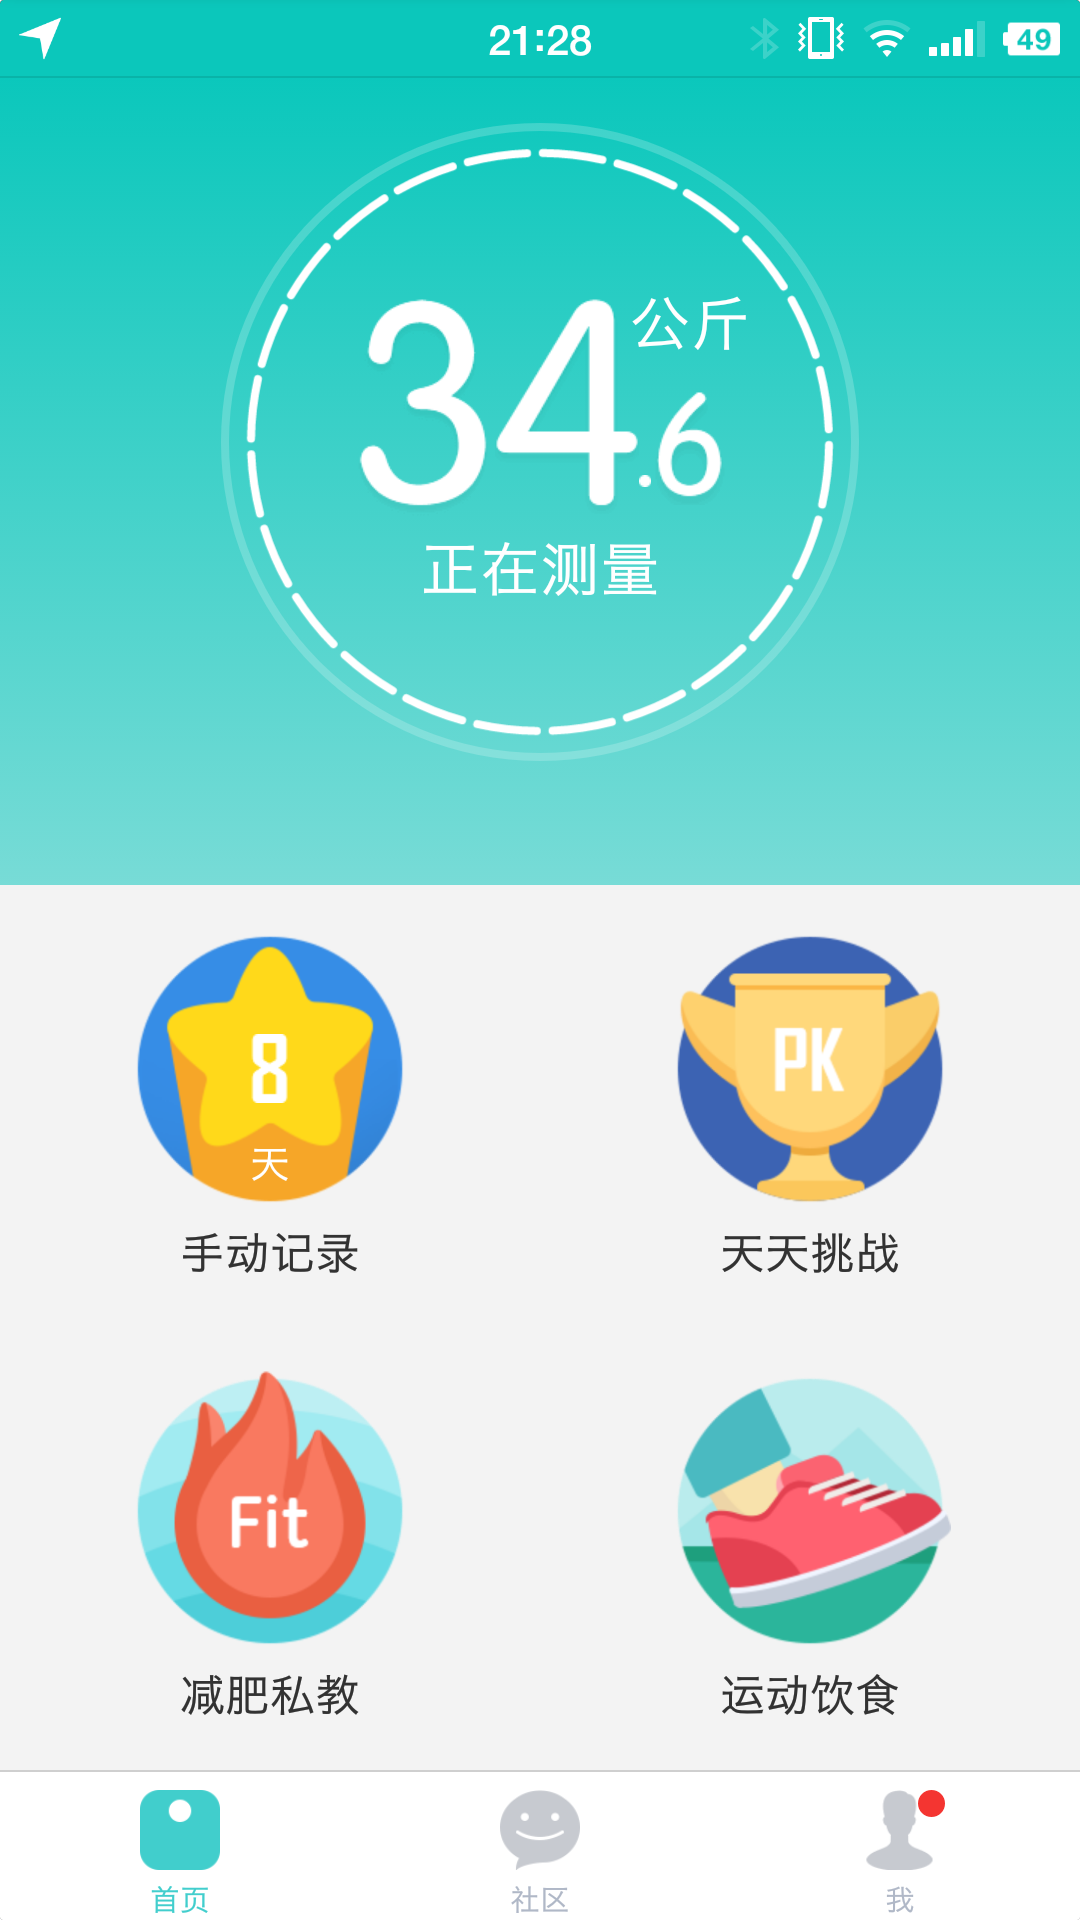
\includegraphics[width=0.6\linewidth]{haoqing-app.png}}
  \end{figure}
  \end{columns}
\end{frame}

\begin{frame}
  \frametitle{YUNMAI Light}
  \begin{columns}
    \column{.5\textwidth}
  \begin{figure}
    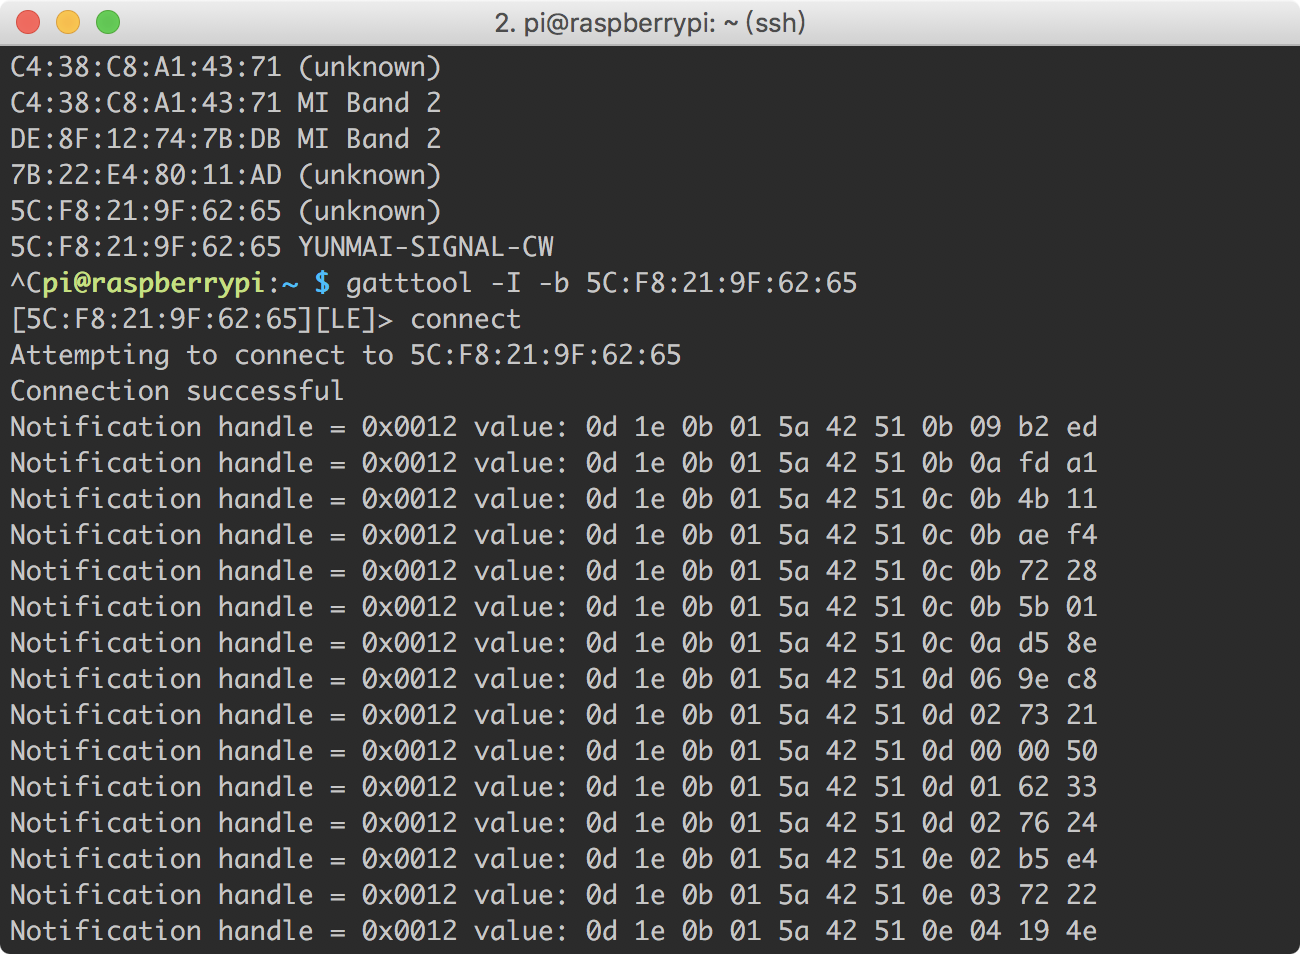
\includegraphics[width=0.9\linewidth]{haoqing-term.png}
  \end{figure}
    \column{.5\textwidth}
  \begin{figure}
    \centering
    \setlength{\fboxrule}{0.001cm}    % 边框线线宽 
    \setlength{\fboxsep}{0}
    \fbox {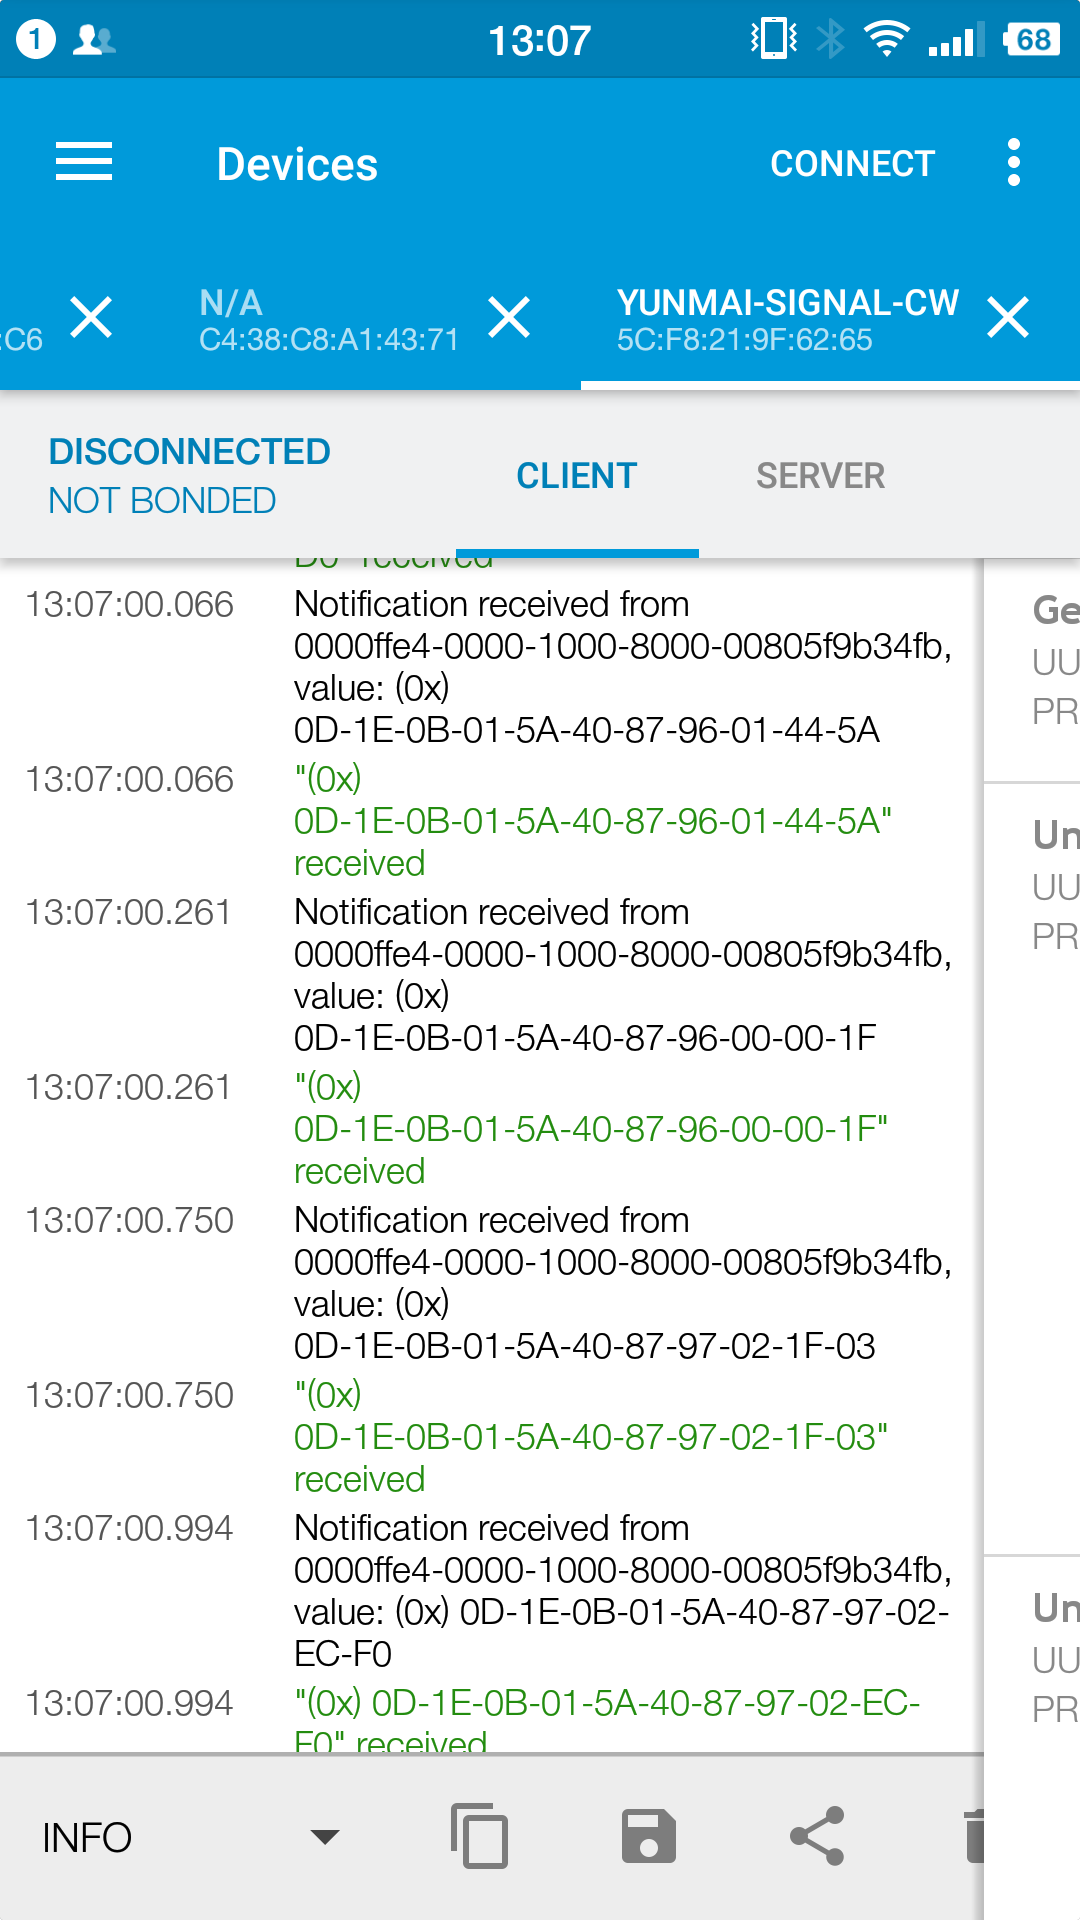
\includegraphics[width=0.6\linewidth]{yunmai-log.png}}
  \end{figure}
  \end{columns}
\end{frame}

\subsection{MI Band 2}

\begin{frame}
  \frametitle{MI Band 2}
  \begin{columns}
    \column{.5\textwidth}
  \begin{figure}
    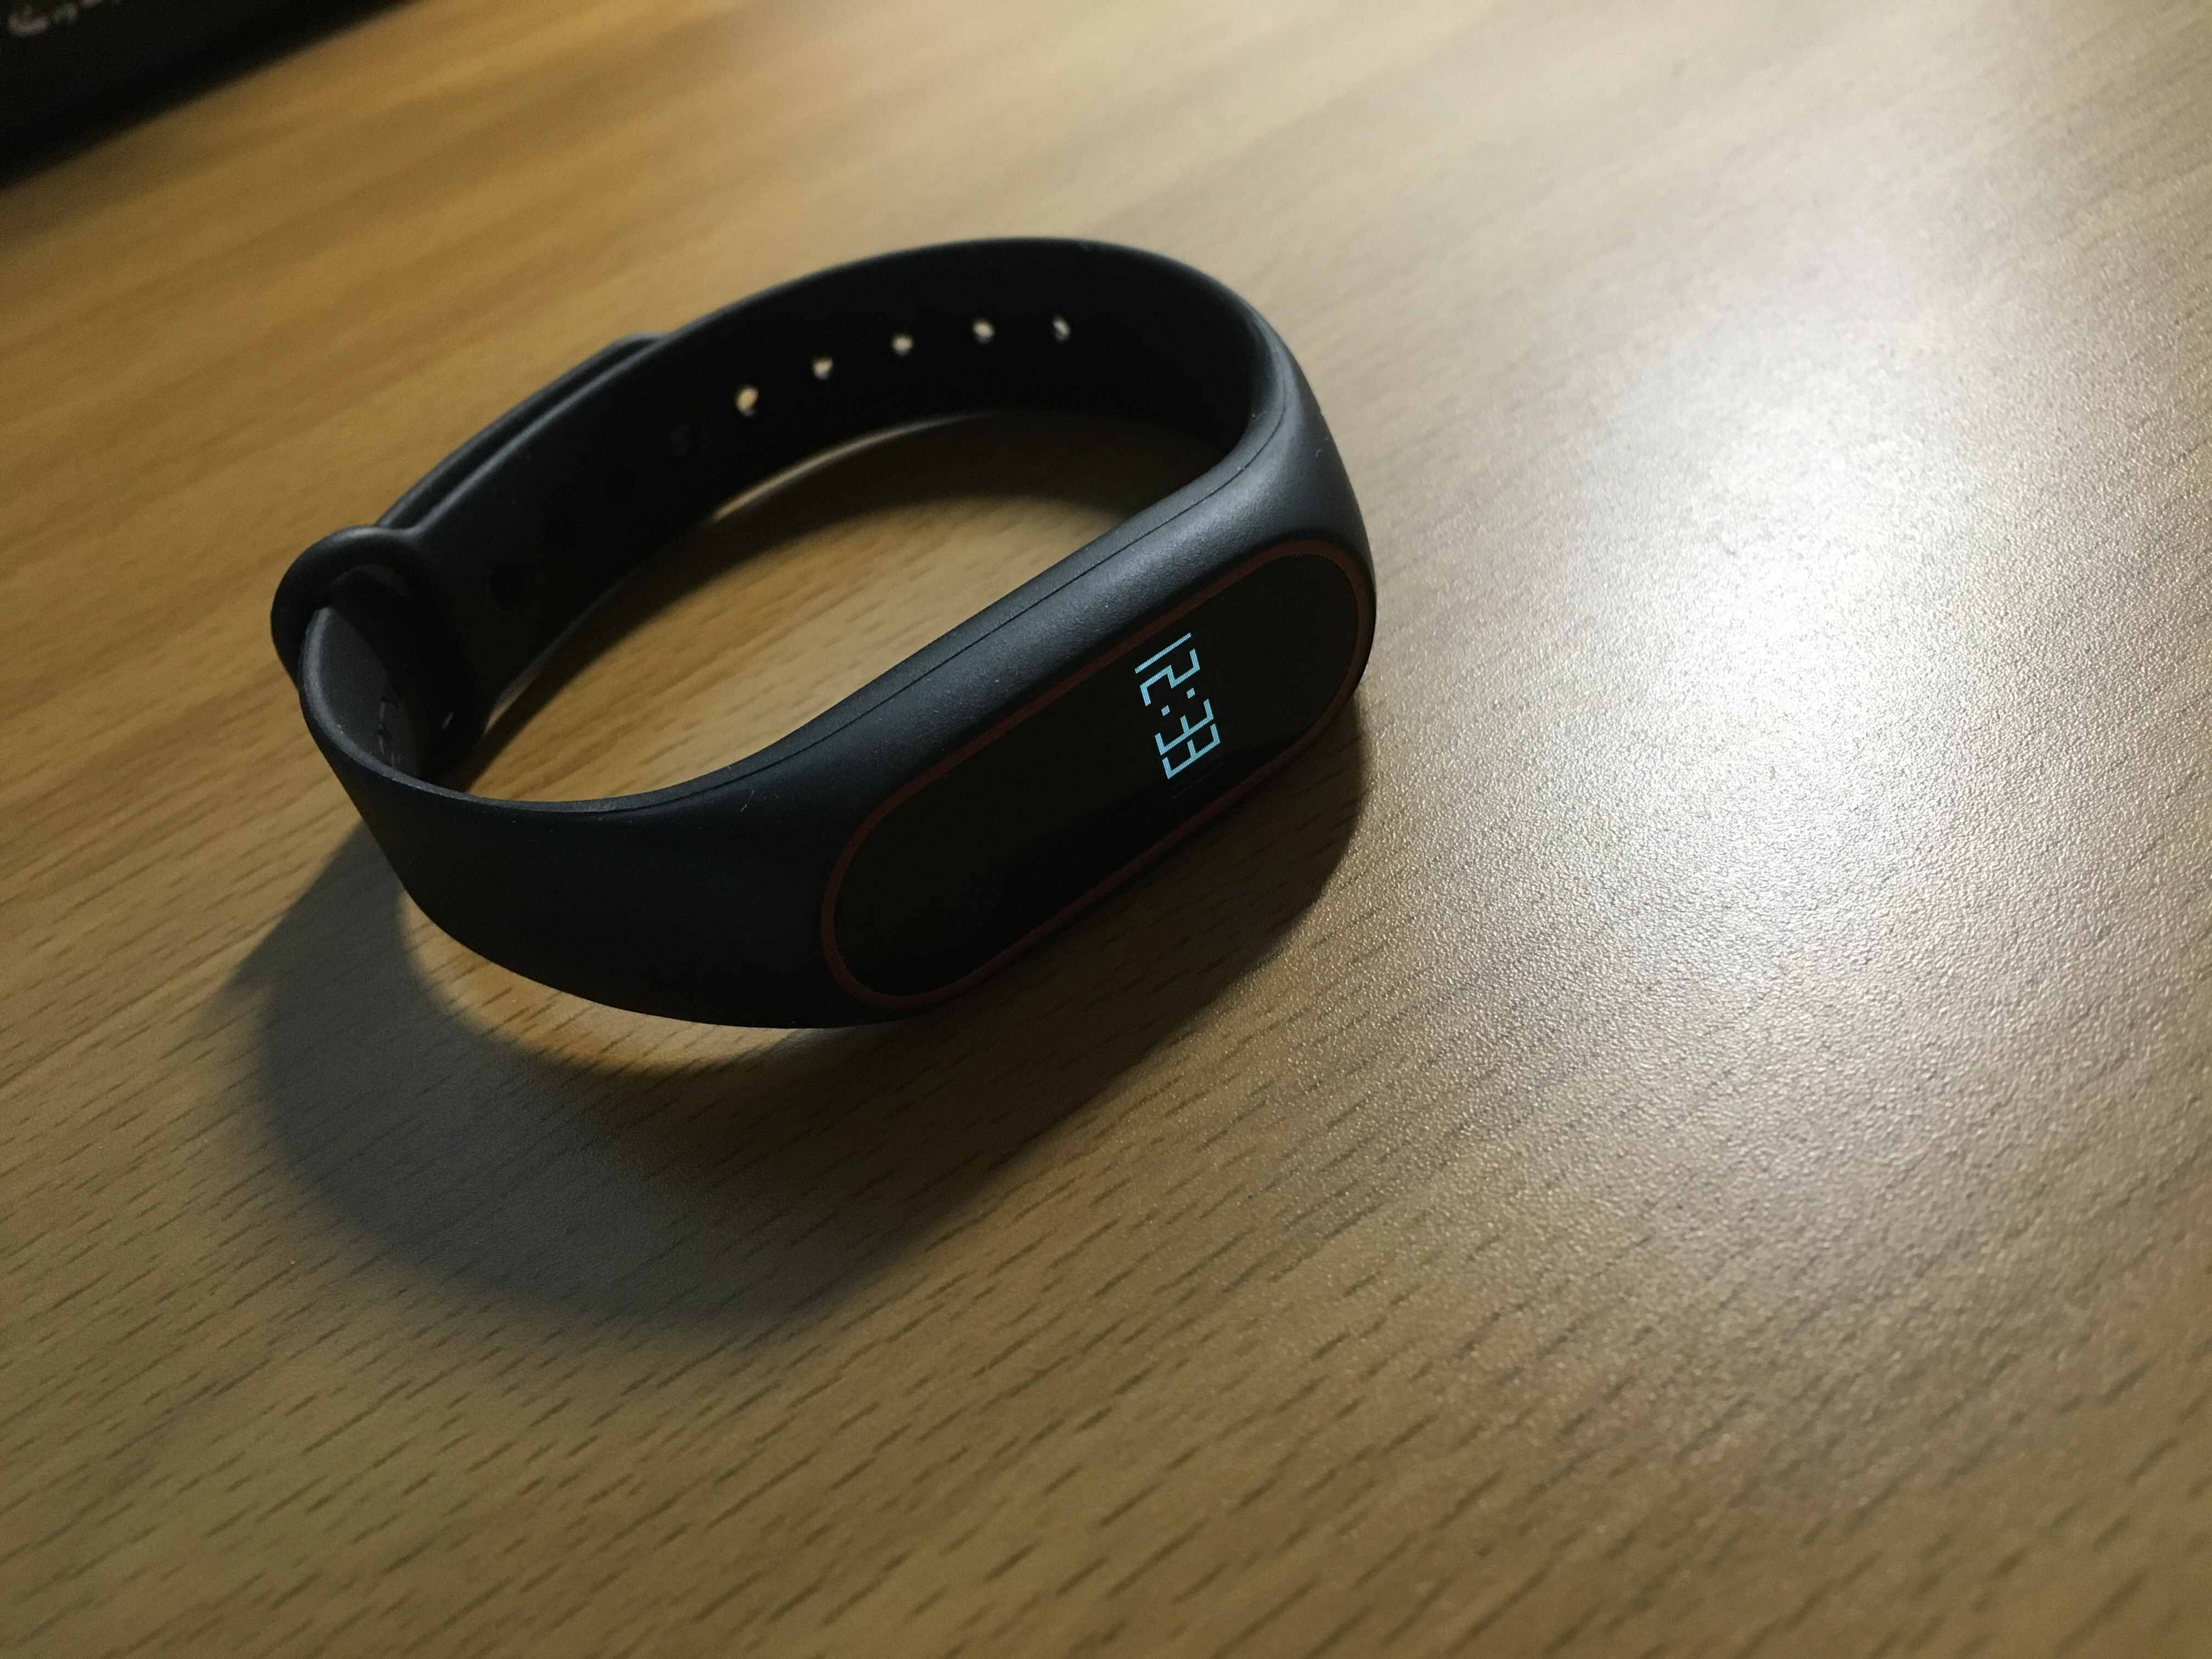
\includegraphics[width=0.9\linewidth]{mi-band-2.jpg}
  \end{figure}
    \column{.5\textwidth}
  \begin{figure}
    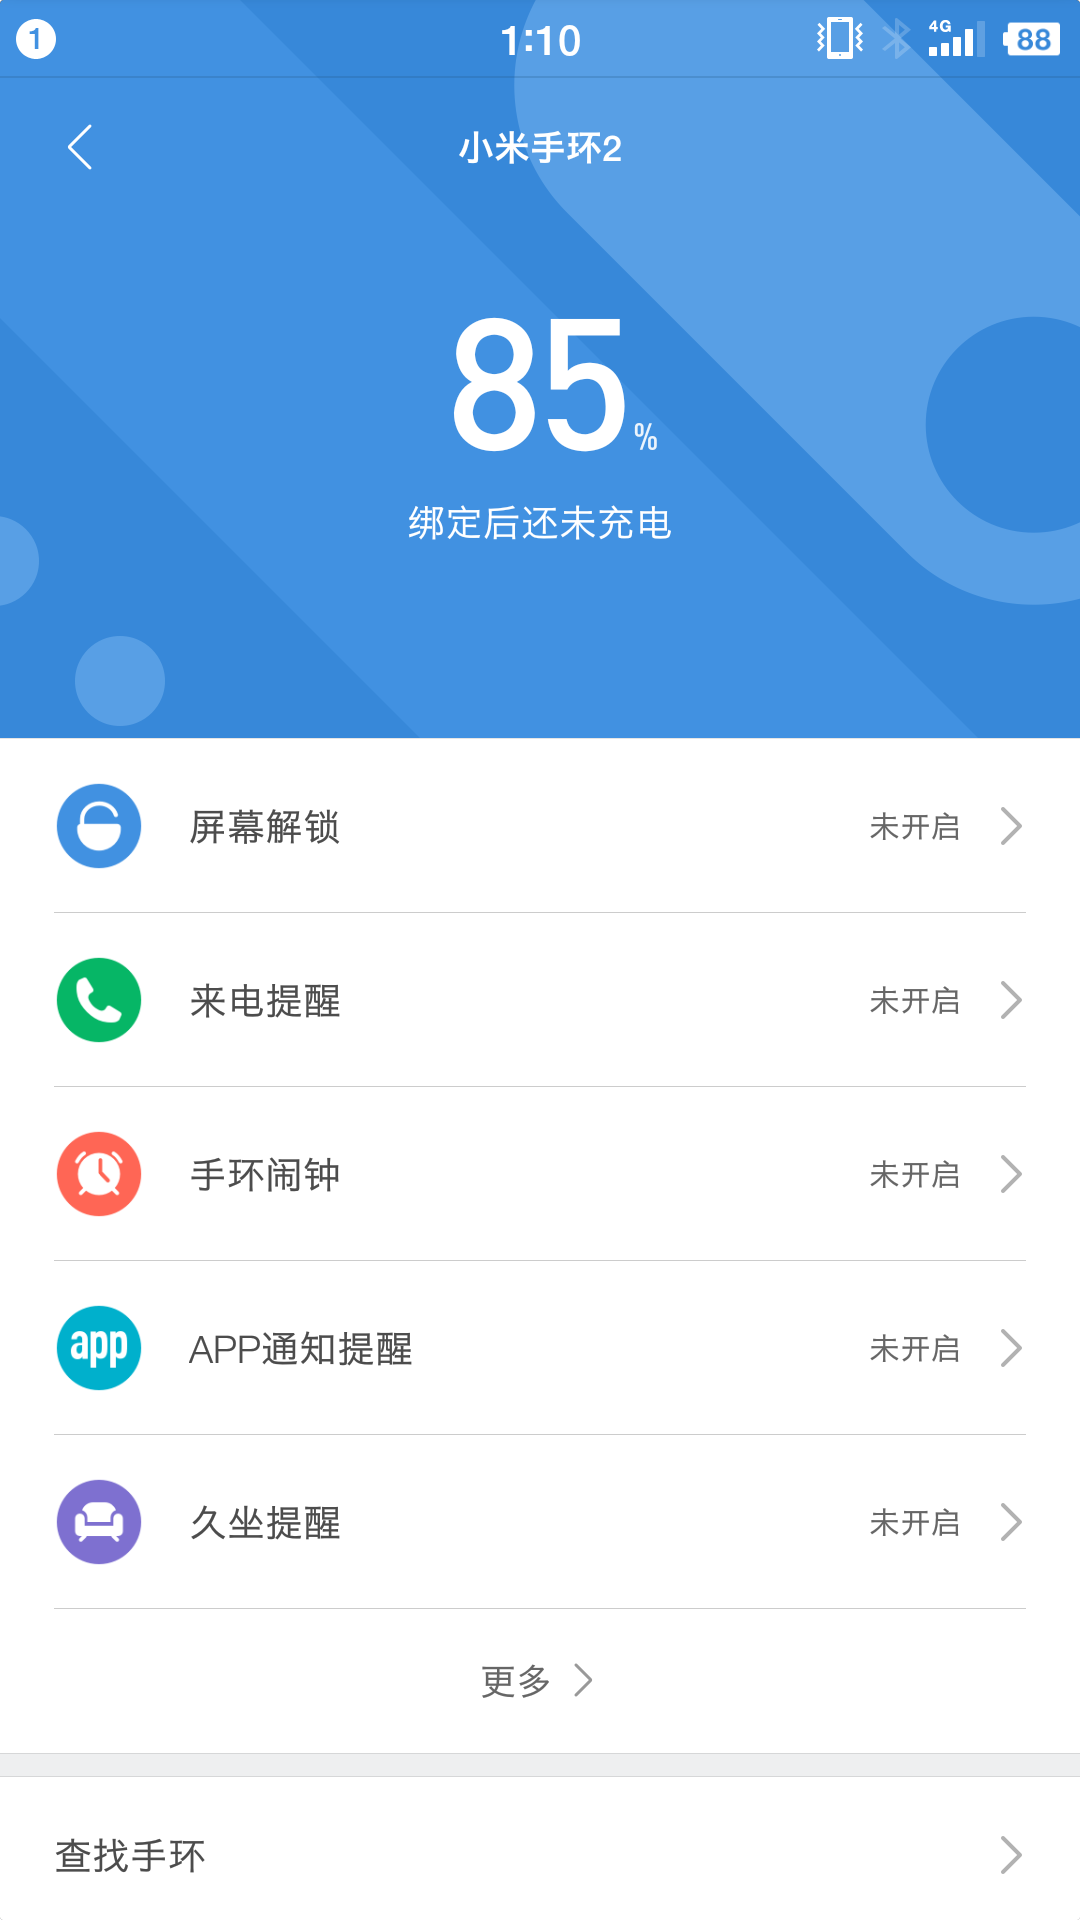
\includegraphics[width=0.6\linewidth]{mi-fit.png}
  \end{figure}
  \end{columns}
\end{frame}

\begin{frame}
  \frametitle{MI Band 2}
  \begin{columns}
    \column{.5\textwidth}
  \begin{figure}
    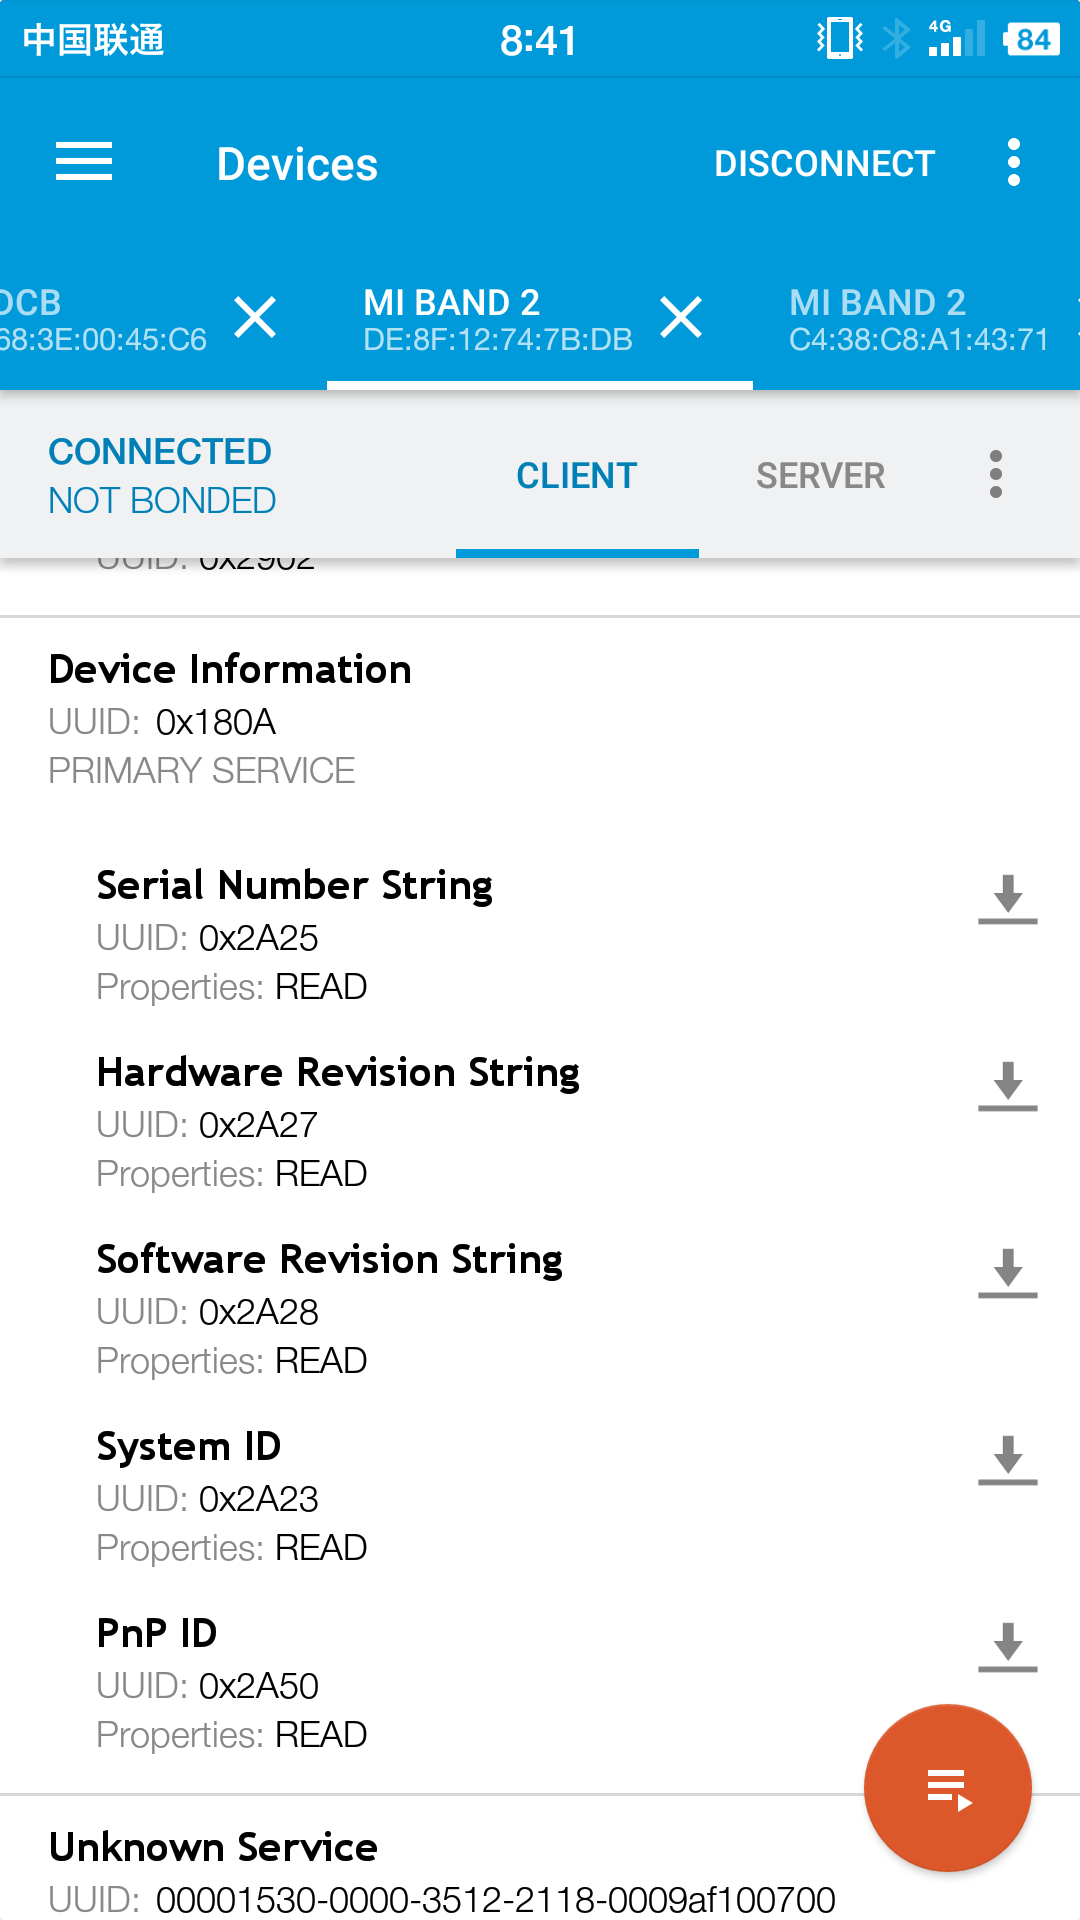
\includegraphics[width=0.6\linewidth]{mi-band-info.png}
  \end{figure}
    \column{.5\textwidth}
  \begin{figure}
    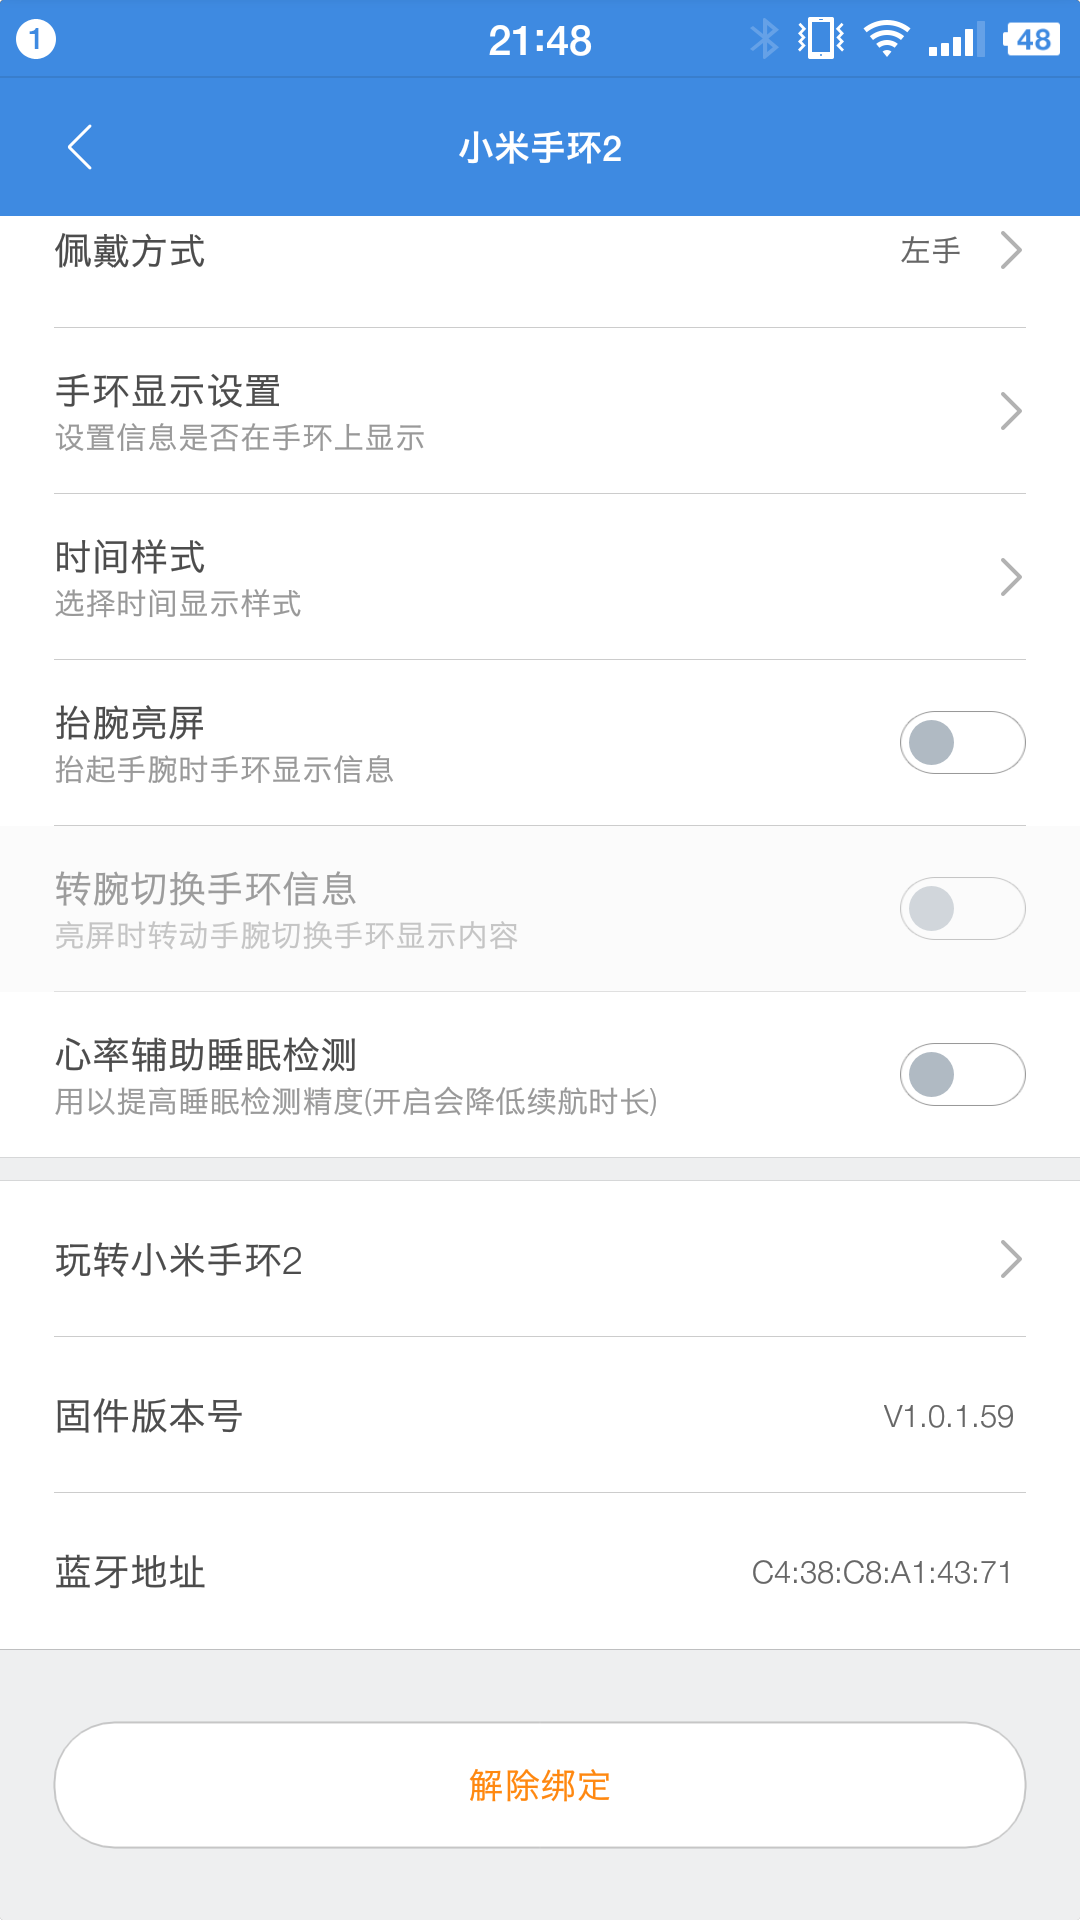
\includegraphics[width=0.6\linewidth]{mifit-app.png}
  \end{figure}
  \end{columns}
\end{frame}

\begin{frame}
  \frametitle{MI Band 2}
  \begin{block}{Basic Service}
    UUID of Service: \\{\Monaco 0000fee0-0000-1000-8000-00805f9b34fb} \\
    Battery Info Characteristic: \\{\Monaco 00000006-0000-3512-2118-0009af100700}
  \end{block}
  \begin{block}{Alert Service}
    UUID of Service: \\{\Monaco 00001802-0000-1000-8000-00805f9b34fb} \\
    New Alert Characteristic: \\{\Monaco 00002a06-0000-1000-8000-00805f9b34fb}
  \end{block}
\end{frame}

\begin{frame}
  \frametitle{MI Band 2}
  \begin{block}{Heart Rate Service}
    UUID of Service: \\{\Monaco 0000180d-0000-1000-8000-00805f9b34fb} \\
    Measurement Characteristic: \\{\Monaco 00002a37-0000-1000-8000-00805f9b34fb} \\
    Control Characteristic: \\{\Monaco 00002a39-0000-1000-8000-00805f9b34fb} \\
    Descriptor: \\{\Monaco 00002902-0000-1000-8000-00805f9b34fb} 
  \end{block}
\end{frame}

\begin{frame}
  \frametitle{MI Band 2}
  \begin{columns}
    \column{.5\textwidth}
  \begin{figure}
    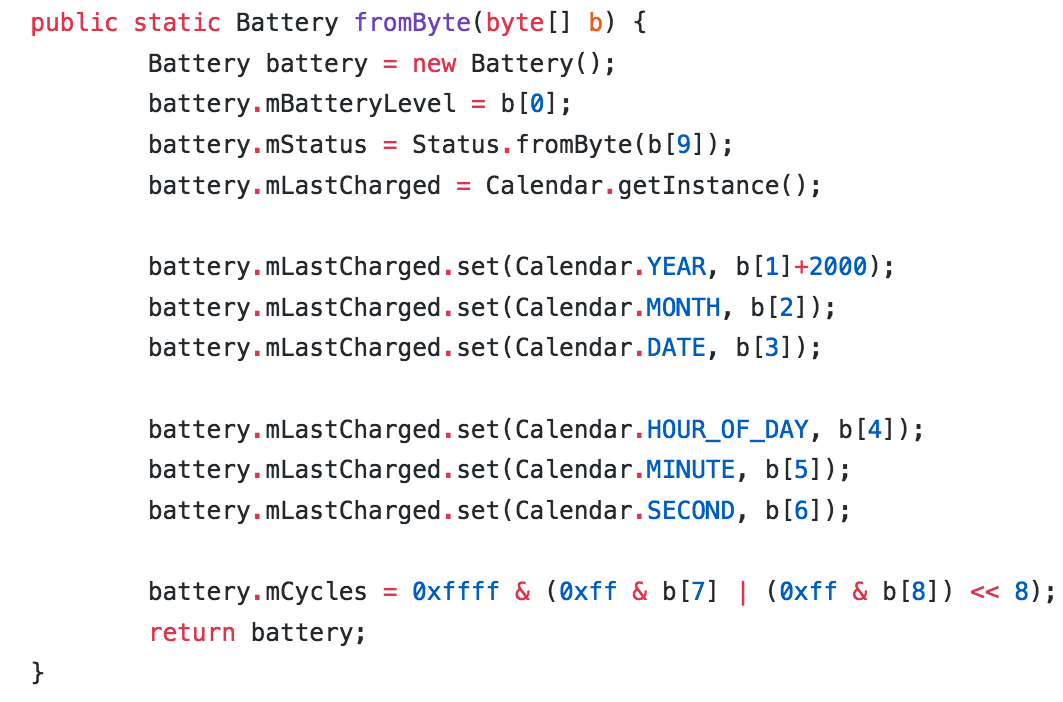
\includegraphics[width=0.9\linewidth]{java.png}
  \end{figure}
    \column{.5\textwidth}
  \begin{figure}
    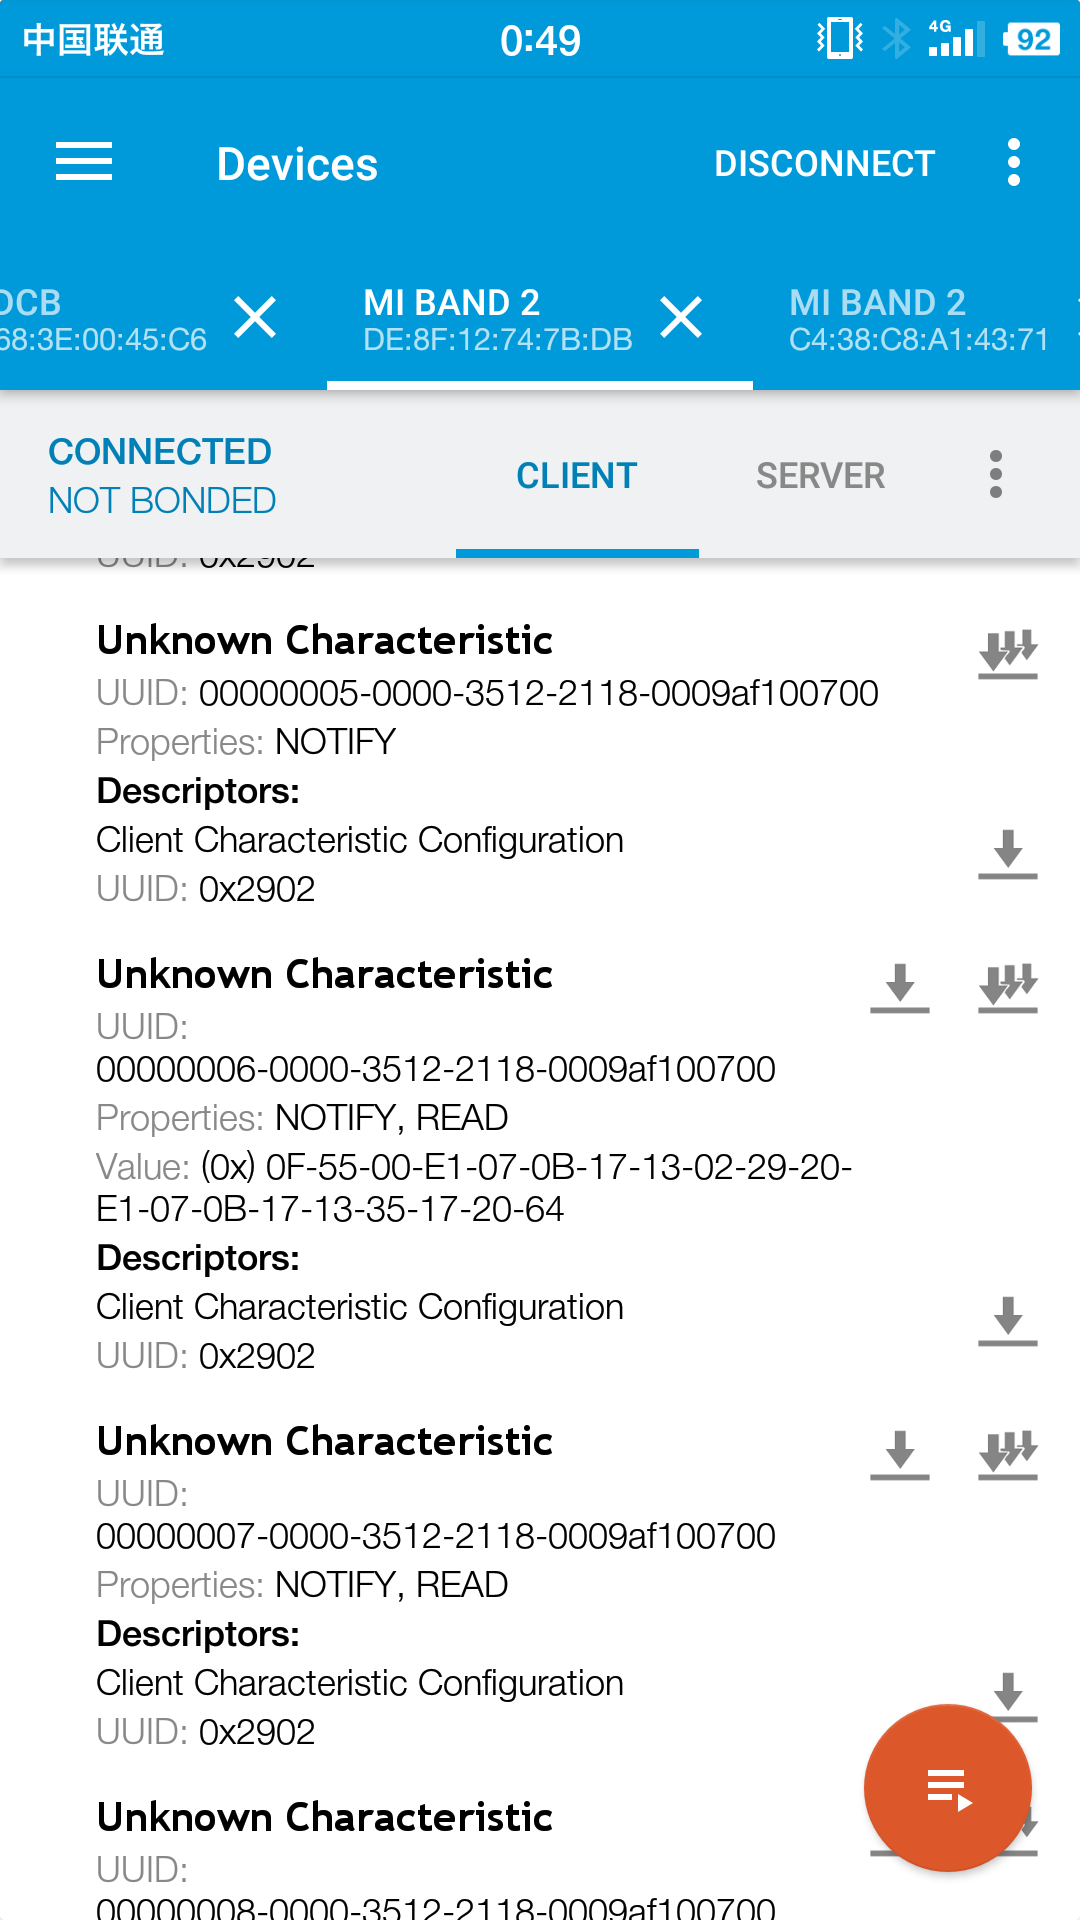
\includegraphics[width=0.6\linewidth]{battery.png}
  \end{figure}
  \end{columns}
\end{frame}

\begin{frame}
  \frametitle{MI Band 2}
   \begin{columns}
    \column{.5\textwidth}
  \begin{figure}
    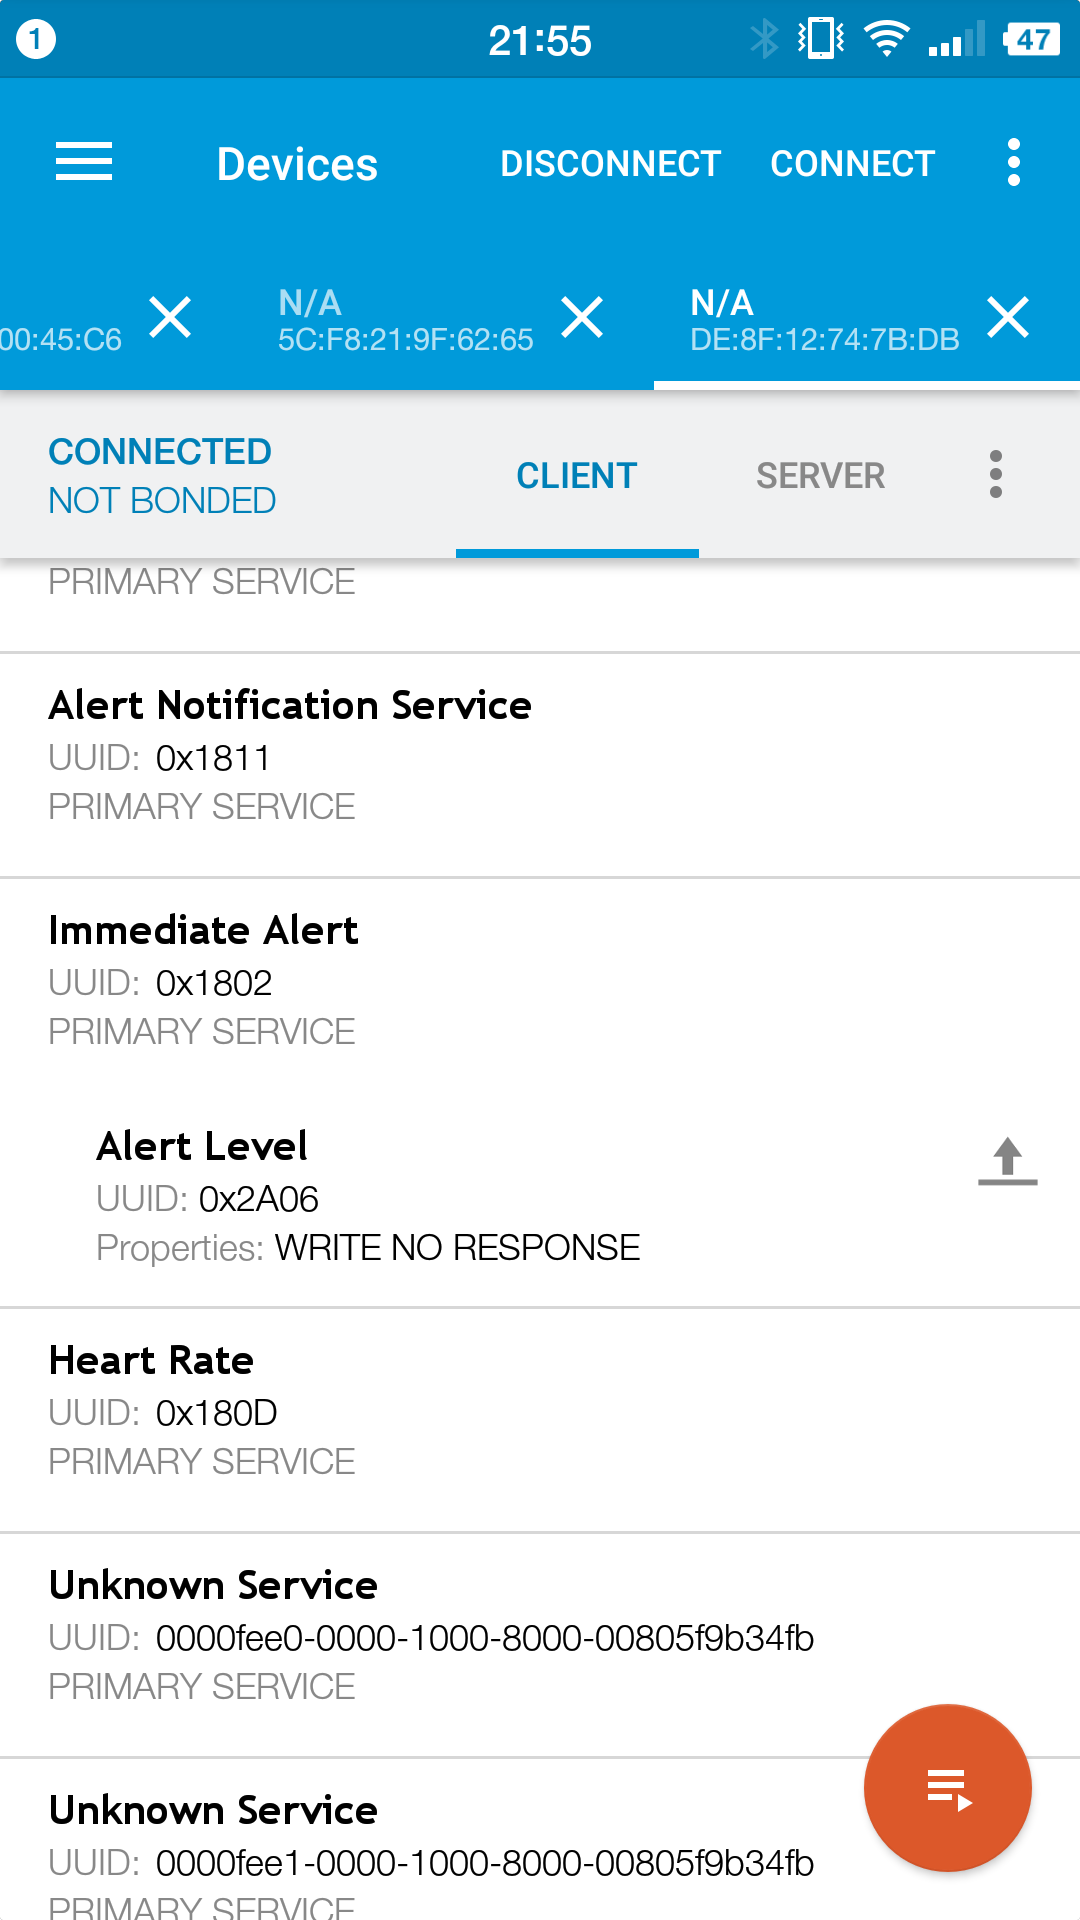
\includegraphics[width=0.6\linewidth]{alert.png}
  \end{figure}
    \column{.5\textwidth}
  \begin{figure}
    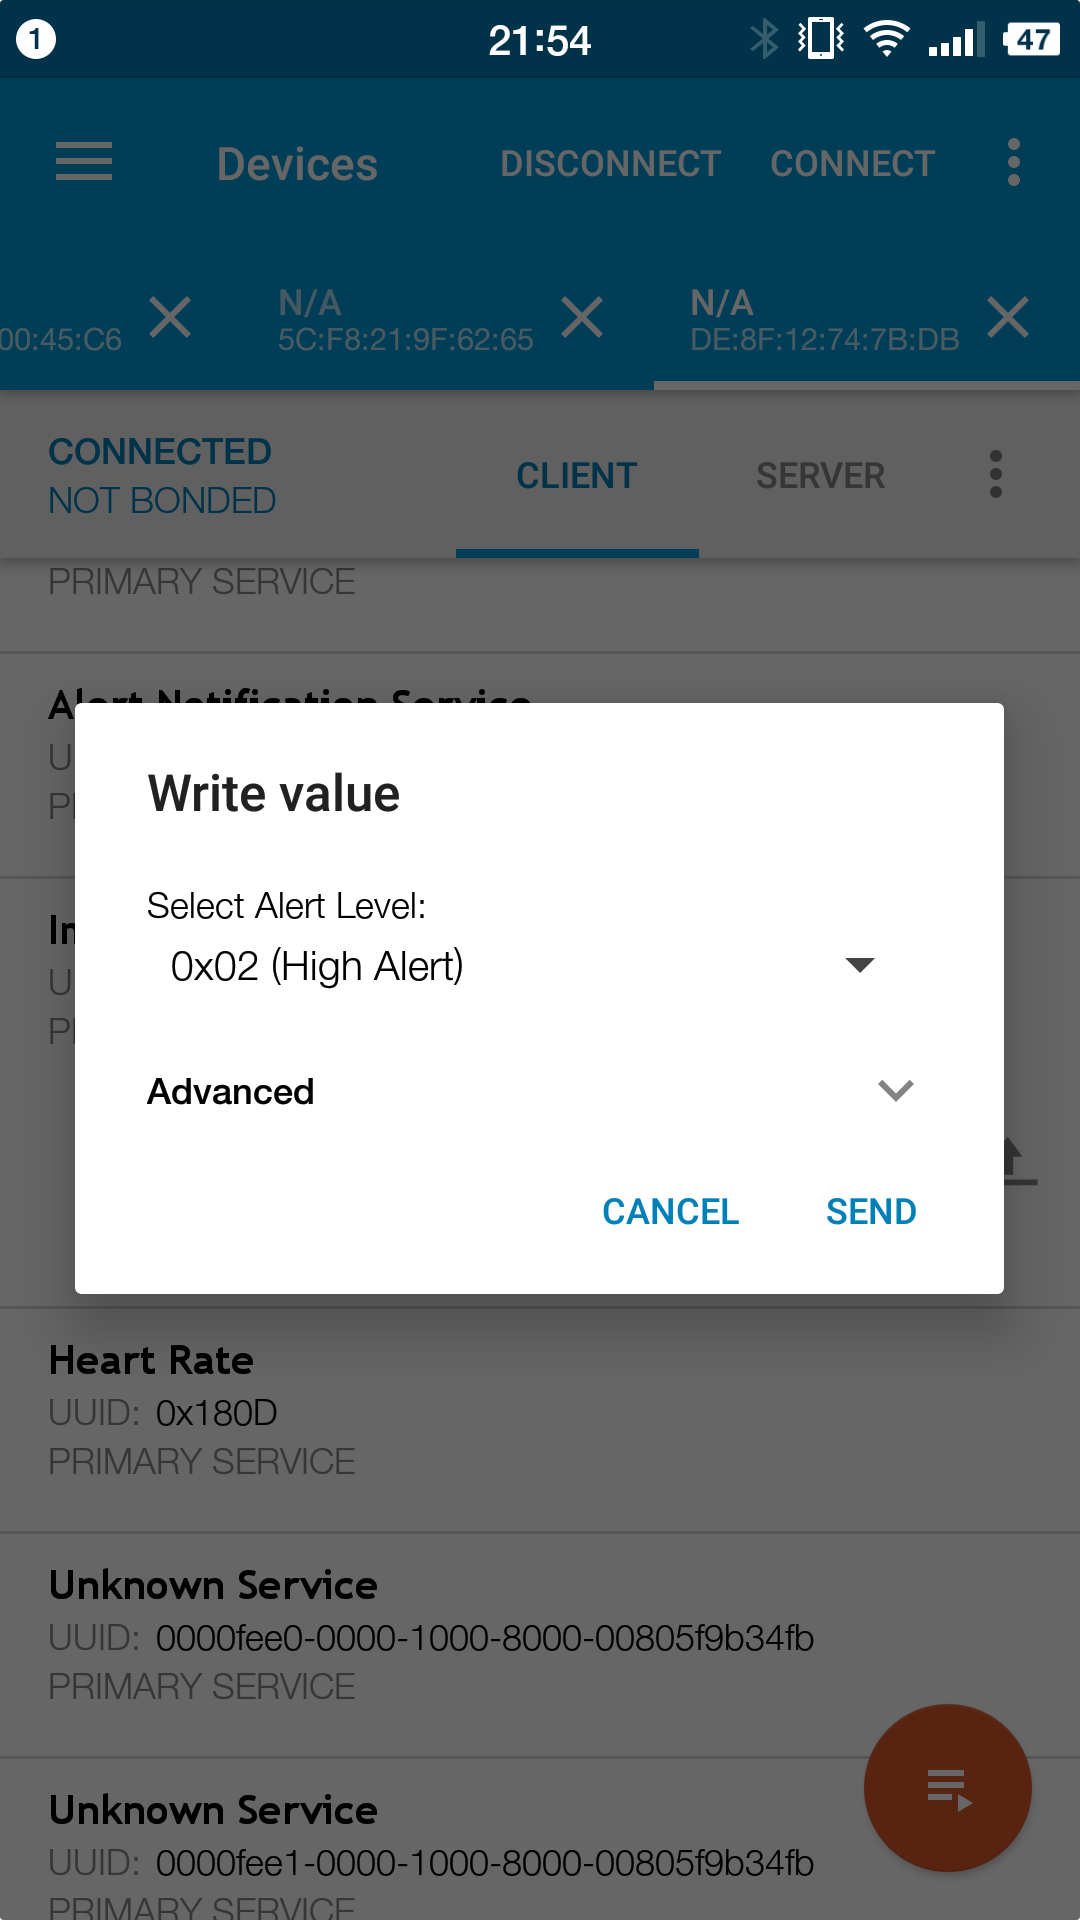
\includegraphics[width=0.6\linewidth]{alert2.png}
  \end{figure}
  \end{columns}
\end{frame}
 

\section{优化方案}

\begin{frame}
	\frametitle{Solution}
	\framesubtitle{Cryptology \& Web Security}
	\begin{figure}
            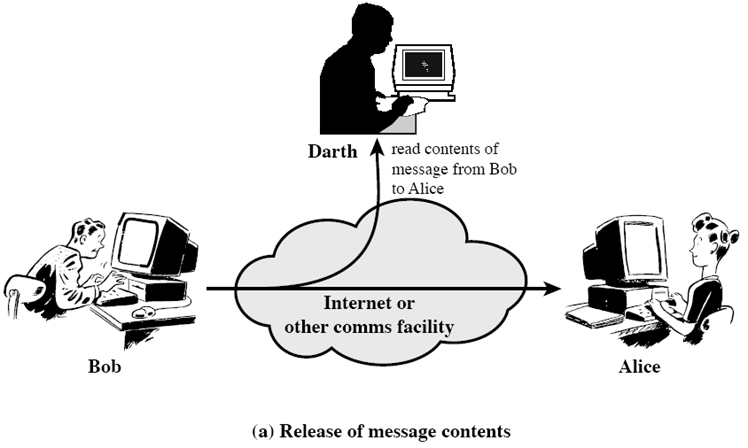
\includegraphics[width=0.6\linewidth]{sniff.png}
	\end{figure}
\end{frame}

\begin{frame}
	\frametitle{Solution}
	\framesubtitle{Cryptology \& Web Security}
	\begin{figure}
            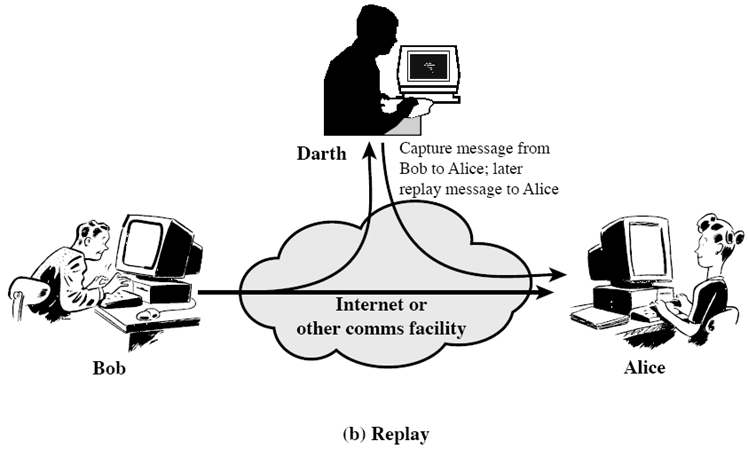
\includegraphics[width=0.6\linewidth]{replay.png}
	\end{figure}
\end{frame}

\begin{frame}
  \frametitle{Solution}
   \begin{columns}
    \column{.5\textwidth}
  \begin{figure}
    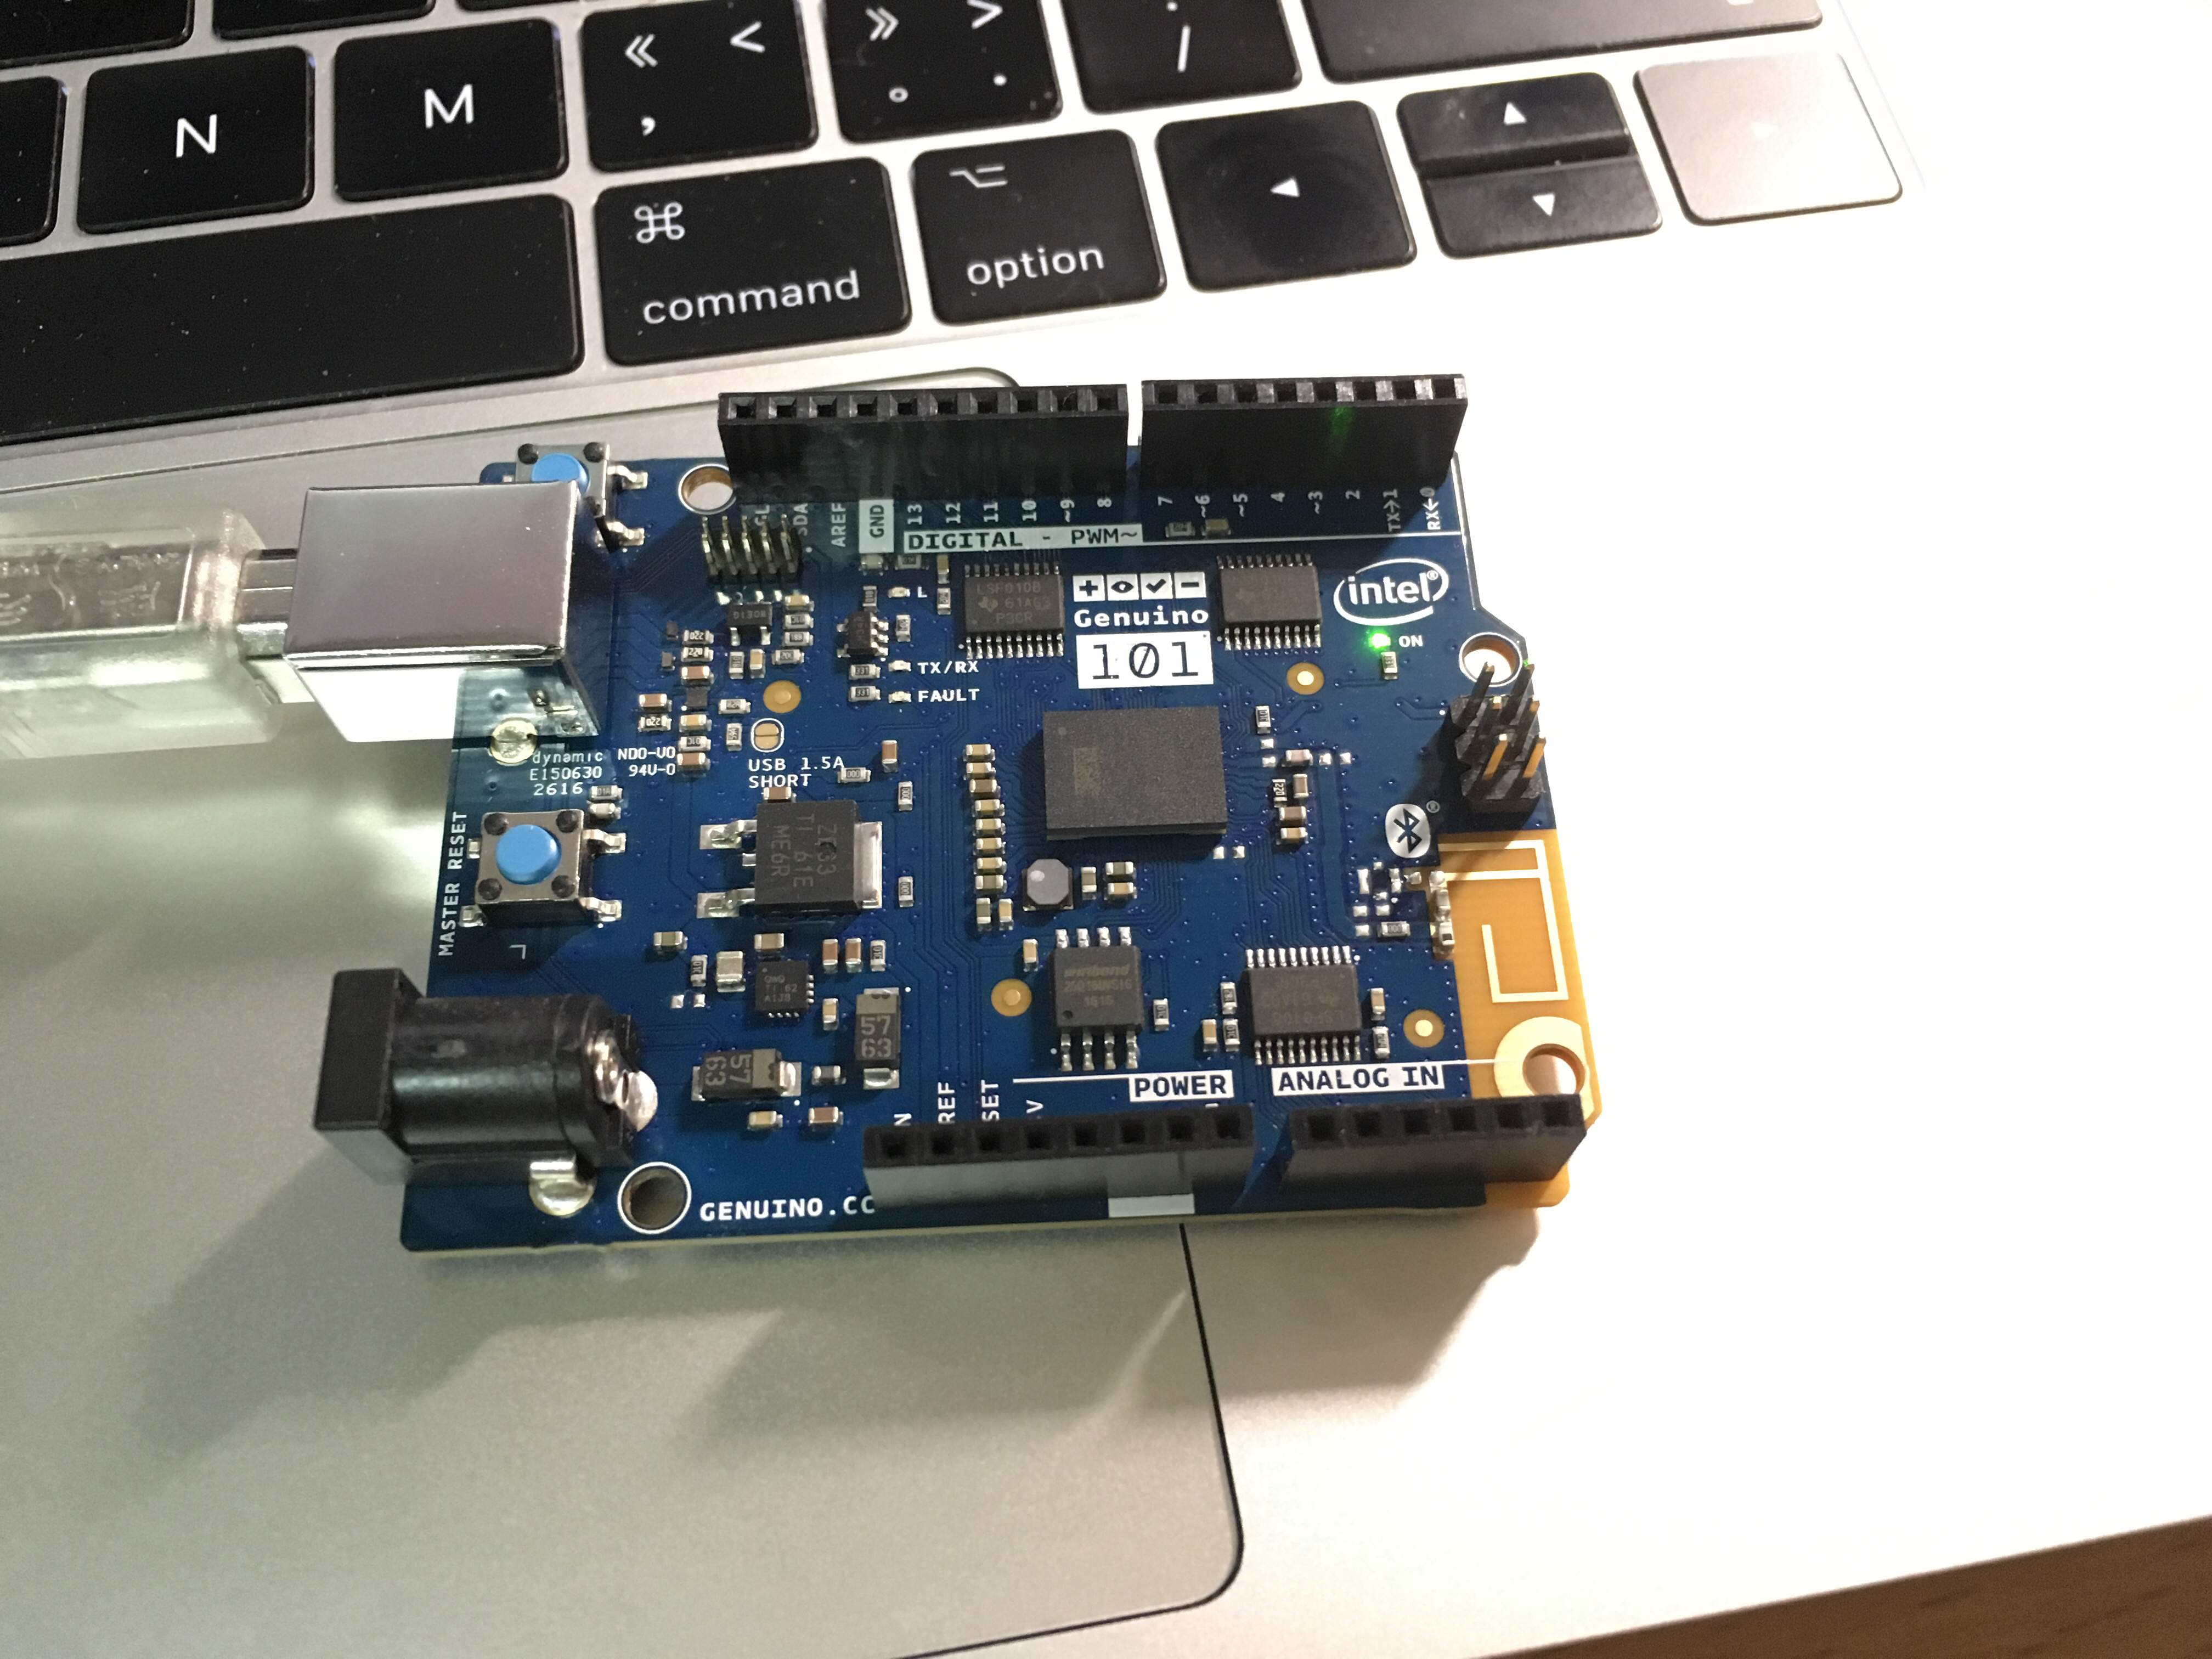
\includegraphics[width=0.9\linewidth]{arduino101.jpg}
  \end{figure}
    \column{.5\textwidth}
  \begin{figure}
    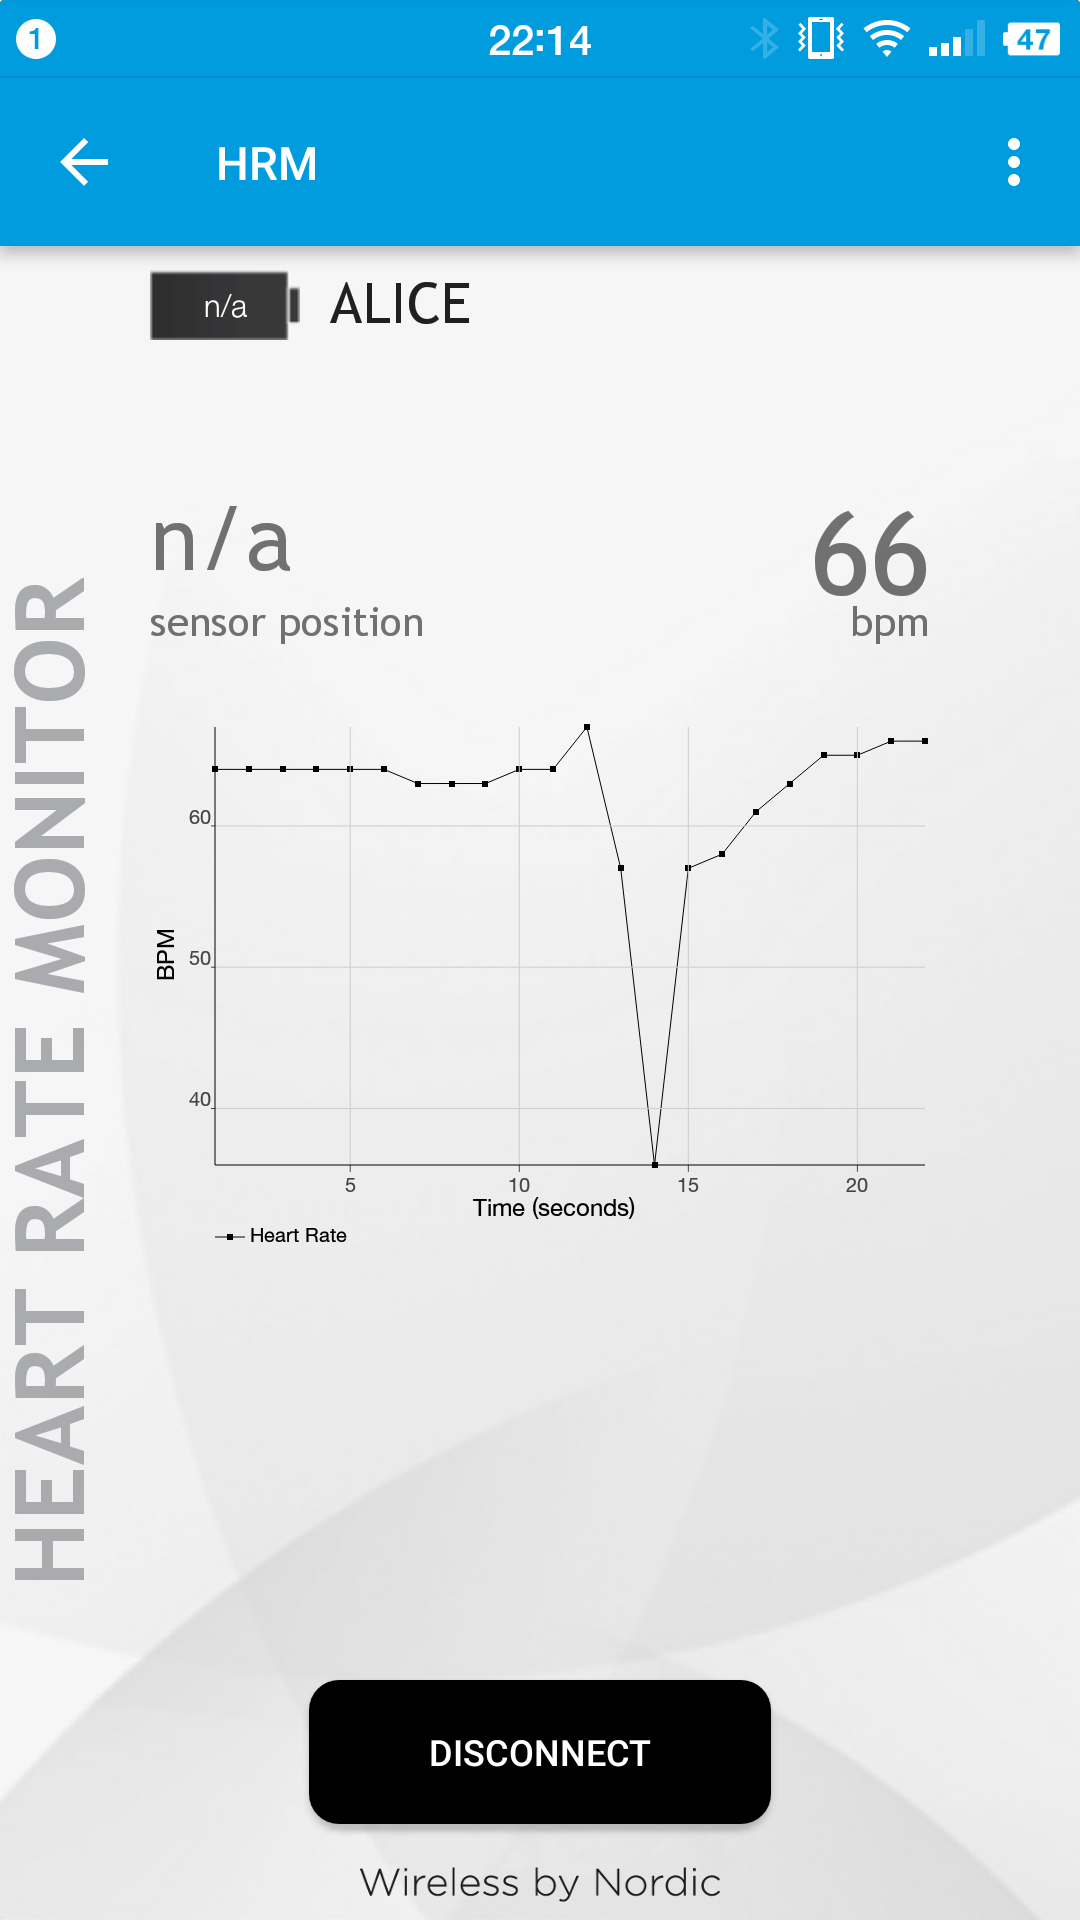
\includegraphics[width=0.6\linewidth]{line.png}
  \end{figure}
  \end{columns}
\end{frame}

\section{结论}

\begin{frame}
  \frametitle{结论}
  \begin{block}{加密和低功耗的冲突}
    运用加密的方式可以有效的防止嗅探攻击,但会增大功耗,与协议设计的初衷相违背,这种冲突是不可避免的。
  \end{block}
  \begin{alertblock}{安全性和低功耗的平衡}
    由于加密与低功耗之间不可避免的冲突,我们应该在安全性与低功耗之间寻找到一个平衡,牺牲一定的功耗来获得一定的安全性,根据不同应用对安全性的需求来考虑应该牺牲多大的功耗。
  \end{alertblock}
\end{frame}

  
\section{参考文献}
\begin{frame}
\frametitle{References}
\footnotesize{
\begin{thebibliography}{99}
\bibitem[Shaikh Shahriar Hassan, Soumik Das Bibon, Md Shohrab Hossain, Mohammed Atiquzzaman]{p1} Shaikh Shahriar Hassan, Soumik Das Bibon, Md Shohrab Hossain, Mohammed Atiquzzaman
\newblock Security threats in Bluetooth technology
\newblock \emph{computers \& security} 2017 doi: 10.1016/j.cose.2017.03.008
\end{thebibliography}
}
\end{frame}

\section{结束语}

\begin{frame}
  \frametitle{End}
\Huge{\centerline{The End}}
\end{frame}

\end{document} 
